\onecolumn
\part*{SUPPLEMENTARY MATERIAL}
\renewcommand{\thesection}{S.\arabic{section}}
\renewcommand{\thesubsection}{S.\arabic{section}.\arabic{subsection}}
\renewcommand{\thesubsubsection}{S.\arabic{section}.\arabic{subsection}%
    .\arabic{subsubsection}}
\renewcommand{\thetable}{S.\arabic{table}}
\renewcommand{\thefigure}{S.\arabic{figure}}
%
%%%%%%%%%%%%%%%%%%%%%%%%%%%%%%%%%%%%%%%%%%%%%%%%%%%%%%%%%%%%%%%%%%%%%%%%%%%%%%%
%<<<<<<< HEAD
%%
%\ifthenelse{\NOT\isundefined{\draft}\OR\NOT\isundefined{\final}}{
{\centering
\subsubsection*{Acronyms}
\printacronyms[heading=none]\par}
%}{}
%%
%\\
%Below we provide the proofs of our results stated in the main part of the paper.
%=======
Below we provide the proofs of the results stated in the main part of the
paper.
%>>>>>>> 1a53644efbc9773324384e46e5d2a47af752482e
\begin{refsection}
\section{Quantile Regression}
\label{appendix:qr}
Let us recall the expression of the pinball loss \seep{figure:pinball}:
\begin{dmath}[compact]
    v_{\hyperparameter}: (y,\,y') \in
    \reals^2 \mapsto  \max{(\hyperparameter (y-y'), (\hyperparameter
    -1)(y-y'))} \in \reals.
\end{dmath}
\begin{floatingfigure}{.7\textwidth}
    \centering
    \begin{tikzpicture}
    \begin{axis}[%
        axis x line = center,
        axis y line = center,
        disabledatascaling,
        axis equal image,
        xlabel = {$y - h(x)$},
        ylabel = {$v_{\theta}(y, h(x))$},
        x label style={at={(axis description cs:1.0, 0.0)}, anchor=north},
        ticks = none
        ]
        \addplot[orange, domain=-1:1, samples at={-1, 0, 1}]
            {abs(.8 - (x < 0)) * abs(x)};
        \draw
            (-0.5, 0.1) coordinate (a)
            (0, 0) coordinate (b)
            (-0.5, 0) coordinate (c);
        \draw
            pic["$\theta - 1$", draw=black, -,dashed, angle eccentricity=1.2,
                angle radius=2.3cm]
            {angle=a--b--c};
        \draw
            (0.5, 0.4) coordinate (d)
            (0, 0) coordinate (e)
            (0.5, 0) coordinate (f);
        \draw
            pic["$\theta$", draw=black, -,dashed, angle eccentricity=1.2,
                angle radius=2.3cm]
            {angle=f--e--d};
    \end{axis}
\end{tikzpicture}

    \caption{\label{figure:pinball} Pinball loss for $\hyperparameter=0.8$.}
\end{floatingfigure}
\begin{proposition}\label{proposition:generalized_excess_risk}
    Let $X,Y$ be two \acp{rv} respectively taking values in $\mcX$ and
    $\reals$, and $q \colon \mcX \to \mathcal{F}([0,1],\mathbb{R})$ the
    associated conditional quantile function.  Let $\mu$ be a positive measure
    on $[0,1]$ such that $ \int_{0}^1 \expectation\left[
    v_{\hyperparameter}\left(Y,q(X)(\hyperparameter)\right)\right] \mathrm{d}
    \mu(\hyperparameter) < \infty$.  Then for $\forall h \in
    \functionspace{\mathcal{X}}{\functionspace{\closedinterval{0}{1}}{\reals}}$
    \begin{dmath*}
        \risk(h) - \risk(q) \geq 0,
    \end{dmath*}
    where $R$ is the risk defined in \cref{equation:h-objective}.
\end{proposition}
\begin{proof}
    The proof is based on the one given in \citep{li2007quantile} for a single
    quantile. Let $f \in
    \functionspace{\mcX}{\functionspace{\closedinterval{0}{1}}{\reals}}$,
    $\hyperparameter \in (0,1)$ and $(x,y) \in \mcX \times \reals$. Let also
    \begin{align*}
        s &=
        \begin{cases}
            1 ~ \text{if } y \leq f(x)(\hyperparameter)      \\
            0  \text{ otherwise}
        \end{cases},&
        t &=
        \begin{cases}
            1 ~ \text{if } y \leq q(x)(\hyperparameter)      \\
            0  \text{ otherwise}
        \end{cases}.
    \end{align*}
    It holds that
    \begin{dmath*}
        v_{\hyperparameter}(y,h(x)(\hyperparameter)) -
        v_{\hyperparameter}(y,q(x)(\hyperparameter))
        = \hyperparameter(1-s)(y-h(x)(\hyperparameter)) + (\hyperparameter -
        1)s(y-h(x)(\hyperparameter)) -
        \hyperparameter(1-t)(y -q(x)(\hyperparameter)) -
        (\hyperparameter-1)t(y-q(x)(\hyperparameter))
        = \hyperparameter(1-t)(q(x)(\hyperparameter) - h(x)(\hyperparameter)) +
        \hyperparameter((1-t)-(1-s))h(x)(\hyperparameter) +
        (\hyperparameter-1)t(q(x)(\hyperparameter - h(x)(\hyperparameter))) +
        (\hyperparameter-1)(t-s)h(x)(\hyperparameter) + (t-s)y\nonumber
        =     (\hyperparameter -t)(q(x)(\hyperparameter) -
        h(x)(\hyperparameter)) +
        (t-s)(y-h(x)(\hyperparameter)).\label{eq:decompo_pinball}
    \end{dmath*}
    Then, notice that
    \begin{dmath*}[compact]
        \expectation{[(\hyperparameter - t)(q(X)(\hyperparameter) -
        h(X)(\hyperparameter))]} =
        \expectation{[\expectation{[(\hyperparameter - t)(q(X)(\hyperparameter)
        - h(X)(\hyperparameter))]} | X]} =
        \expectation{[\expectation{[(\hyperparameter - t) | X ]}
        (q(X)(\hyperparameter) - h(X)(\hyperparameter))]}
    \end{dmath*}
    and since $q$ is the true quantile function,
    \begin{align*}
        \expectation{ [t | X]} = \expectation{ [\mathbf{1}_{\{ Y \leq
        q(X)(\hyperparameter)\}} | X]} = \probability{[Y \leq
        q(X)(\hyperparameter) | X]} = \hyperparameter,
    \end{align*}
    so
    \begin{align*}
        \expectation{[(\hyperparameter - t)(q(X)(\hyperparameter) -
        h(X)(\hyperparameter))]} =0.
    \end{align*}
    Moreover, $(t-s)$ is negative when $q(x)(\hyperparameter) \leq y \leq
    h(x)(\hyperparameter)$, positive when $h(x)(\hyperparameter) \leq y \leq
    q(x)(\hyperparameter)$ and $0$ otherwise, thus the quantity
    $(t-s)(y-h(x)(\hyperparameter))$ is always positive. As a consequence,
    \begin{dmath*}[compact]
        R(h) - R(q) = \int_{[0,1]}
        \expectation{[v_{\hyperparameter}(Y,h(X)(\hyperparameter)) -
        v_{\hyperparameter}(Y,q(X)(\hyperparameter))]} \mathrm{d}
        \mu(\hyperparameter) \geq 0
    \end{dmath*}
    which concludes the proof.
\end{proof}
The \cref{proposition:generalized_excess_risk} allows us to derive conditions
under which the minimization of the risk above yields the true quantile
function. Under the assumption that (i) $q$ is continuous (as seen as a
function of two variables), (ii) $\mathrm{Supp}(\mu) = [0,1] $, then the
minimization of the integrated pinball loss performed in the space of
continuous functions yields the true quantile function on the support of
$\probability_{X,Y}$.


\section{Representer Propositions}
\label{appendix:representer}
\begin{proof} [Proof of \cref{theorem:representer_supervised}]
    First notice that
    \begin{align}
        J: h \in \mcH_K \mapsto \frac{1}{n} \displaystyle\sum_{i=1}^n
        \displaystyle\sum_{j=1}^m w_j\hcost(\hyperparameter_j,y_i,
        h(x_i)(\hyperparameter_j)) + \frac{\lambda}{2} \norm{h}_{\mcH_K}^2 \in
        \reals
    \end{align}
    is a proper lower semicontinuous strictly convex function
    \citep[Corollary 9.4]{bauschke2011convex}, hence $J$ admits a unique
    minimizer $h^* \in \mcH_K$ \citep[Corollary 11.17]{bauschke2011convex}.
    Let
    \begin{dmath}[compact] \label{decompo_theorem}
        \mcU = \sspan{ \Set{
        (K(\cdot,x_i)k_{\Theta}(\cdot,\theta_j))_{i,j=1}^{n,m} | \forall  x_i
        \in \inputspace , \forall \theta_j \in \hyperparameterspace }} \subset
        \mcH_K.
    \end{dmath}
    Then $\mcU$ is a finite-dimensional subspace of $\mcH_K$, thus closed in
    $\mcH_K$, and it holds that $\mcU \oplus \mcU^{\perp} = \mcH_K$, so $h^*$
    can be decomposed as $h^* = h_{\mcU}^* + h_{\mcU^{\perp}}^*$ with
    $h_{\mcU}^* \in \mcU$ and $h_{\mcU^{\perp}}^* \in \mcU^{\perp}$. Moreover,
    for all $1 \leq i \leq n$ and $1 \leq j \leq m$,
    \begin{align*}
        h_{\mcU^{\perp}}^*(x_i)(\theta_j) &= \langle h_{\mcU^{\perp}}^*(x_i) ,
        k_{\Theta}(\cdot,\theta_j) \rangle_{\mcH_{k_{\Theta}}}
        = \langle h_{\mcU^{\perp}}^* , K(\cdot,x_i)k_{\Theta}(\cdot,\theta_j)
        \rangle_{\mcH_K}
        = 0,
    \end{align*}
    so $J(h^*) = J(h_{\mcU}^*) + \lambda \norm{h_{\mcU^{\perp}}^*}_{\mcH_K}^2$.
    However $h^*$ is the minimizer of J, therefore $h_{\mcU^{\perp}}^*=0$ and
    there exist $\left(\alpha_{ij}\right)_{i,j = 1}^{n,m}$ such that $\forall
    x,\hyperparameter \in \mcX \times \hyperparameterspace$,
    $h^*(x)(\hyperparameter) = \sum_{i,j=1}^{n,m} \alpha_{ij} k_{\mcX}(x,x_i)
    k_{\hyperparameterspace}(\hyperparameter,\hyperparameter_j)$.
    % Remark \citep{carmeli06vector} that $\mcH_K$ is isometric to the real RKHS
    %  $\mcH_{k_{\mcX}\times k_{\Theta}}$ thanks to the isometry
    %  \begin{dmath*}
    %    V \colon
    %    \begin{cases}
    %        \mcH_K & \to ~ \mcH_{k_{\mcX}\times k_{\Theta}}       \\
    %        h  & \mapsto (x,\theta \mapsto h(x)(\theta))
    %    \end{cases}
    %  \end{dmath*}
    %   Let $g^* = V(h^*)$, and define
    %   \begin{dmath*}[compact]
    %   \mcV = \sspan{ \left \{
    %   (k_{\mcX}(x_i,\cdot)k_{\Theta}(\theta_j,\cdot))_{i,j=1}^{n,m} \right \}}
    %   \subset \mcH_{k_{\mcX}\times k_{\Theta}}
    %   \end{dmath*}
      % $\mcU$ is a finite dimensional subspace of $\mcH_{k_{\mcX}\times k_{\Theta}}$,
      % thus closed, and $\mcV \oplus \mcV^{\perp} = \mcH_{k_{\mcX}\times k_{\Theta}}$,
      % so that we can write $g^* = g_{\mcV}^* + g_{\mcV^{\perp}}^*$ with $g_{\mcV}^* \in \mcV$
      % and $g_{\mcV^{\perp}}^* \in \mcV^{\perp}$. By construction,
      % \begin{dmath*}
      %   \widetilde{R}_{\mcS}(h^*) = \frac{1}{nm} \sum_{i,j=1}^{n,m}
      %   \parametrizedcost{\hyperparameter_j}(y,h^*(x_i)(\hyperparameter_j)) +
      %    \lambda \norm{h^*}_{\mcH_K}^2
      %   =\frac{1}{nm} \sum_{i,j=1}^{n,m}
      %    \parametrizedcost{\hyperparameter_j}(y,g^*(x_i,\hyperparameter_j)) +
      %    \lambda \norm{g^*}_{\mcH_{k_{\mcX}\times k_{\Theta}}}^2
      %    = \frac{1}{nm} \sum_{i,j=1}^{n,m}
      %    \parametrizedcost{\hyperparameter_j}(y,g_{\mcV}^*(x_i,\hyperparameter_j)) +
      %    \lambda (\norm{g_{\mcV}^*}_{\mcH_{k_{\mcX}\times k_{\Theta}}}^2 +
      %    \norm{g_{\mcV^{\perp}}^*}_{\mcH_{k_{\mcX}\times k_{\Theta}}}^2)
      % \end{dmath*}
      % since
    \paragraph{Derivative shapes constraints:}
    Reminder: for a function $h$ of one variable, we denote $\partial h$ the
    derivative of $h$. For a function $k(\theta, \theta')$ of two variables we
    denote $\partial_1 k$ the derivative of $k$ with respect to $\theta$ and
    $\partial_2 k$ the derivative of $k$ with respect to $\theta'$.
    %
    From \citet{zhou2008derivative}, notice that if $f\in\mathcal{H}_k$, where
    $\mathcal{H}_k$ is a scalar-valued \ac{RKHS} on a compact subset
    $\hyperparameterspace$ of $\reals^d$, and $k\in
    \mathcal{C}^{2}(\hyperparameterspace \times \hyperparameterspace)$ (in the
    sense of \citet{ziemer2012weakly}) then $\partial f\in\mathcal{H}_k$. Hence
    if one add a new term of the form:
    \begin{dmath*}
        \lambda_{\text{nc}} \sum_{i=1}^n\sum_{j=1}^m \Omega_{\text{nc}}
        \left(\left(\partial\left[h(x_i)\right]\right)(\theta_j)\right) =
        \lambda_{\text{nc}}\sum_{i=1}^n\sum_{j=1}^m
        \Omega_{\text{nc}}\left((\partial h(x_i))(\theta_j)\right)
    \end{dmath*}
    where $g$ is a strictly monotonically increasing function and
    $\lambda_{\text{nc}} > 0$, a new representer theorem can be obtained by
    constructing the new set
    \begin{dmath*}[compact] 
        \mcU = \sspan{ \Set{
        (K(\cdot,x_i)k_{\Theta}(\cdot,\theta_j))_{i,j=1}^{n,m} | \forall  x_i
        \in \inputspace , \forall \theta_j \in \hyperparameterspace }
        \cup \Set{
        (K(\cdot,x_i)(\partial_2 k_{\Theta})(\cdot,\theta_j))_{i,j=1}^{n,m} |
        \forall  x_i \in \inputspace , \forall \theta_j \in
        \hyperparameterspace }
        }
        \subset
        \mcH_K.
    \end{dmath*}
    The proof is the same as \cref{theorem:representer_supervised} with the
    new set $\mathcal{U}$ to obtain the expansion $h(x)(\theta) =
    \sum_{i=1}^n\sum_{j=1}^m \alpha_{ij} k_{\inputspace}(x,
    x_i)k_{\hyperparameterspace}(\theta, \theta_j) + \beta_{ij}k(x,
    x_i)(\partial_2k_{\hyperparameterspace})(\theta, \theta_j)$.  For the
    regularization notice that for a symmetric function $(\partial_1 k)(\theta,
    \theta') = (\partial_2 k)(\theta', \theta)$. Hence $\inner{(\partial_1
    k)(\cdot, \theta'), k(\cdot, \theta)}_{\mathcal{H}_k} = \inner{k(\cdot,
    \theta'), (\partial_2 k)(\cdot, \theta)}_{\mathcal{H}_k}$ and $(\partial
    k_{\theta'})(\theta) = (\adjoint{\partial} k_{\theta})(\theta')$ and
    \begin{dmath*}
        \norm{h}_{\mathcal{H}_K}^2
        = \inner{h, h}_{\mathcal{H}_K}
        = \sum_{i=1}^n\sum_{j=1}^m\sum_{i'=1}^n\sum_{j'=1}^m
        \alpha_{ij}\alpha_{i'j'}k_{\inputspace}(x_i,
        x_{i'})k_{\hyperparameterspace}(\theta_j, \theta_{j'}) +
        \alpha_{ij}\beta_{i'j'}k_{\inputspace}(x_i, x_{i'})(\partial_2
        k_{\hyperparameterspace})(\theta_j, \theta_{j'}) +
        \alpha_{i'j'}\beta_{ij}k_{\inputspace}(x_i, x_{i'})(\partial_1
        k_{\hyperparameterspace})(\theta_j, \theta_{j'}) +
        \beta_{ij}\beta_{i'j'}k_{\inputspace}(x_i,
        x_{i'})(\partial_1\partial_2k_{\hyperparameterspace})(\theta_j,
        \theta_{j'})
    \end{dmath*}
    Eventually $(\partial h(x))(\theta) = \sum_{i=1}^n\sum_{j=1}^m \alpha_{ij}
    k_{\inputspace}(x, x_i)(\partial_1 k_{\hyperparameterspace})(\theta,
    \theta_j) + \beta_{ij}k(x,
    x_i)(\partial_1\partial_2k_{\hyperparameterspace})(\theta, \theta_j)$.
\end{proof}
To prove \cref{theorem:representer_ocsvm}, the following lemmas are useful.
\begin{lemma} \citep{carmeli10vector} \label{lemma:isometry}
    Let $k_{\mcX}:\inputspace \times \inputspace \rightarrow \reals$,
    $k_{\hyperparameterspace}:\hyperparameterspace \times \hyperparameterspace
    \rightarrow \reals$ be two scalar-valued kernels and $K (\theta',\theta) =
    k_{\hyperparameterspace}(\theta,\theta')I_{\mcH_{k_{\mcX}}}$.  Then $H_K$
    is isometric to $\mcH_{k_{\mcX}} \otimes \mcH_{k_{\hyperparameterspace}}$
    by means of the isometry $W: f \otimes g \in \mcH_{k_{\mcX}} \otimes
    \mcH_{k_{\hyperparameterspace}} \mapsto ( \hyperparameter \mapsto
    g(\hyperparameter)f) \in \mcH_K$.
\end{lemma}
%
\begin{remark}
    Given $k_{\mcX}:\inputspace \times \inputspace \rightarrow \reals$,
    $k_{\hyperparameterspace}:\hyperparameterspace \times \hyperparameterspace
    \rightarrow \reals$ two scalar-valued kernels, we define $K:(x,z) \in \mcX
    \times \mcX \mapsto k_{\mcX}(x,z) I_{\mcH_{k_{\hyperparameterspace}}} \in
    \mathcal{L}(\mcH_{k_{\hyperparameterspace}}  )$, $K':
    (\hyperparameter,\hyperparameter')\in \hyperparameterspace \times
    \hyperparameterspace \mapsto
    k_{\hyperparameterspace}(\hyperparameter,\hyperparameter')
    I_{\mcH_{k_{\mcX}}} \in \mathcal{L}(\mcH_{k_{\mcX}})$.
    \cref{lemma:isometry} allows us to say that $\mcH_{K}$ and $\mcH_{K'}$ are
    isometric by means of the isometry \begin{align}
    \label{equation:v_definition} W: h \in \mcH_{K'} \mapsto (x \mapsto (\theta
    \mapsto h(\theta)(x))) \in \mcH_K.  \end{align}
\end{remark}

\begin{lemma} \label{lemma:decompo_ortho}
    Let $k_{\mcX}:\inputspace \times \inputspace \rightarrow \reals$,
    $k_{\hyperparameterspace}:\hyperparameterspace \times \hyperparameterspace
    \rightarrow \reals$  be two scalar-valued kernels and $K : (\theta,\theta')
    \mapsto k_{\hyperparameterspace}(\theta,\theta')I_{\mcH_{k_{\mcX}}}$.  For
    $\hyperparameter \in \hyperparameterspace$, define $K_{\hyperparameter}: f
    \in \mcH_{k_{\mcX}} \mapsto \left ( \hyperparameter' \mapsto
    K(\hyperparameter',\hyperparameter)f \right ) \in \mcH_K$.  It is easy to
    see that $K_{\hyperparameter}^*$ is the evaluation operator
    $K_{\hyperparameter}^*: h \in \mcH_K \mapsto h(\hyperparameter) \in
    \mcH_{k_{\mcX}}$.  Then $\forall m \in \mathbb{N}^*, \forall
    (\theta_j)_{j=1}^m \in \Theta^m$,
    \begin{dmath} \label{equation:decompo_ortho}
        \left ( +_{j=1}^m \Image(K_{\theta_j}) \right) \oplus \left
        (\cap_{j=1}^m \Nullspace(K_{\theta_j} ^*) \right ) = \mcH_K
    \end{dmath}
\end{lemma}
\begin{proof}
    The statement boils down to proving that $\mcV :=\left ( +_{j=1}^m
    \Image(K_{\theta_j}) \right)$ is closed in $\mcH_K$, since it is
    straightforward that $\mcV ^{\perp} = \left (\cap_{j=1}^m \Nullspace
    \left(K_{\theta_j} ^*\right ) \right)$.  Let  $\left(e_j \right)_{j=1}^k$
    be an orthonormal basis of
    $\sspan{\Set{(k_{\hyperparameterspace}(\cdot,\hyperparameter_j))_{j=1}^m}}
    \subset \mcH_{k_{\hyperparameterspace}}$. Such basis can be obtained by
    applying the Gram-Schmidt orthonormalization method to
    $(k_{\hyperparameterspace}(\cdot,\hyperparameter_j))_{j=1}^m$. Then, $V =
    \sspan{ \Set{ e_j \cdot f , 1 \leq j \leq k, f \in \mcH_{k_{\mcX}}}}$.
    Notice also that $1 \leq j,l \leq k, \forall f,g \in \mcH_{k_{\mcX}}$,
    \begin{dmath} \label{equation:scalar_tensor} \langle e_j \cdot f, e_l \cdot
    g \rangle_{\mcH_K} = \langle e_j , e_l
    \rangle_{\mcH_{k_{\hyperparameterspace}}} \cdot \langle f,g
    \rangle_{\mcH_{k_{\mcX}}} \end{dmath} Let $(h_n)_{n \in \mathbb{N}^*}$ be a
    sequence in $\mcV$ converging to some $h \in \mcH_K$. By definition, one
    can find sequences $(f_{1,n})_{n \in \mathbb{N}^*},\ldots,(f_{k,n})_{n \in
    \mathbb{N}^*} \in \mcH_{k_{\mcX}}$ such that $\forall n \in \mathbb{N}^*$,
    $h_n = \sum_{j=1}^k e_j \cdot f_{n,j}$.  Let $p,q \in \mathbb{N}^*$. It
    holds that, using the orthonormal property of $\left(e_j \right)_{j=1}^k$
    and \cref{equation:scalar_tensor}, $\norm{h_p - h_q}_{\mcH_K}^2 = \norm{
    \sum_{j=1}^k e_j (f_{j,p} - f_{j,q})}_{\mcH_K}^2 = \sum_{j=1}^k \norm{
    f_{j,p} - f_{j,q}}_{\mcH_{k_{\mcX}}}^2$. $(h_n)_{n \in \mathbb{N}^*}$ being
    convergent, it is a Cauchy sequence, thus so are the sequences
    $(f_{j,n})_{n \in \mathbb{N}^*}$. But $\mcH_{k_{\mcX}}$ is a complete
    space, so these sequences are convergent in $\mcH_{k_{\mcX}}$, and by
    denoting $f_j = \lim_{n \to \infty} f_{j,n}$, one gets $h = \sum_{j=1}^k
    e_k \cdot f_j$.  Therefore $h \in \mcV$, $\mcV$ is closed and the
    orthogonal decomposition \cref{equation:decompo_ortho} holds.
\end{proof}
%
\begin{lemma} \label{lemma:coercivity}
    Let $k_{\mcX},k_{\hyperparameterspace}$ be two scalar kernels and $K :
    (\theta,\theta') \mapsto
    k_{\hyperparameterspace}(\theta,\theta')I_{\mcH_{k_{\mcX}}}$.  Let also $m
    \in \mathbb{N}^*$ and $(\theta_j)_{j=1}^m \in \Theta^m$, and $\mcV = \left
    ( +_{j=1}^m \Image(K_{\theta_j}) \right)$. Then  $I: \mcV \rightarrow
    \reals$ defined as $I (h) =  \sum_{j=1}^m
    \norm{h(\hyperparameter_j)}_{\mcH_{k_{\mcX}}}^2$ is coercive.
\end{lemma}
\begin{proof}
    Notice first that if there exists $\theta_j$ such that
    $k_{\hyperparameterspace}(\theta_j,\theta_j) = 0$, then
    $\Image(K_{\theta_j})=0 $, so without loss of generality, we assume that
    $k_{\hyperparameterspace}(\theta_j,\theta_j) > 0 $ ($1 \leq j \leq m$).
    Notice that $I$ is the quadratic form associated to the $L:\mcH_K
    \rightarrow \mcH_K$ linear mapping $ L (h) = \sum_{j=1}^m
    K_{\hyperparameter_j}K_{\hyperparameter_j}^*$.  Indeed, $\forall h \in
    \mcV$, $I(h) = \sum_{j=1}^m \langle
    K_{\hyperparameter_j}^*h,K_{\hyperparameter_j}^*h \rangle_{\mcH_{k_{\mcX}}}
    = \sum_{j=1}^m \langle h, K_{\hyperparameter_j}K_{\hyperparameter_j}^* h
    \rangle_{\mcH_K} = \langle h , L h \rangle_{\mcH_K}$.  Moreover, $\forall 1
    \leq j \leq m$, $K_{\hyperparameter_j}K_{\hyperparameter_j}^*$ has the same
    eigenvalues as $K_{\hyperparameter_j}^*K_{\hyperparameter_j}$, and $\forall
    f \in \mcH_{k_{\mcX}}$, $K_{\hyperparameter_j}^*K_{\hyperparameter_j} f =
    k_{\hyperparameterspace}(\hyperparameter_j,\hyperparameter_j)f$, so that
    the only possible eigenvalue is
    $k_{\hyperparameterspace}(\hyperparameter_j,\hyperparameter_j)$.  Let $h
    \in \mcV$, $h \neq 0$. Because of the \cref{equation:decompo_ortho}, $h$
    cannot be simultaneously in all $\Nullspace(K_{\hyperparameter_j}^*)$, and
    there exists $i_0$ such that $I(h) \geq
    k_{\hyperparameterspace}(\hyperparameter_{i_0},\hyperparameter_{i_0})
    \norm{h}_{\mcH_K}^2$.  Let $\gamma = \underset{1 \leq j \leq m}{\min}
    k_{\hyperparameterspace}(\hyperparameter_{j},\hyperparameter_{j})$.  By
    assumption $\gamma >0$, and it holds that $\forall h \in \mcV$, $I(h) \geq
    \gamma \norm{h}_{\mcH_K}^2$, which proves the coercivity of $I$.
\end{proof}
\begin{proof} [Proof of \cref{theorem:representer_ocsvm}]
    Let $K: (x,z) \in \mcX \times \mcX \mapsto k_{\mcX}(x,z)
    I_{\mcH_{k_{\hyperparameterspace}}} \in
    \mathcal{L}(\mcH_{k_{\hyperparameterspace}}  )$, $K':
    (\hyperparameter,\hyperparameter') \in \hyperparameterspace \times
    \hyperparameterspace \mapsto
    k_{\hyperparameterspace}(\hyperparameter,\hyperparameter')
    I_{\mcH_{k_{\mcX}}} \in \mathcal{L}(\mcH_{k_{\mcX}})$, and define
    \begin{dmath*}
        J \colon
        \begin{cases}
            \mcH_K \times \mcH_{k_{b}} & \to \mathbb{R}  \\
            (h,t)  & \mapsto   \frac{1}{n} \displaystyle\sum_{i,j=1}^{n,m}
            \frac{w_j}{\hyperparameter_j} \abs{t(\hyperparameter_j) -
            h(x_i)(\hyperparameter_j)}_{+} + \displaystyle\sum_{j=1}^m w_j
            \left (\norm{h(\cdot)(\hyperparameter_j)}_{\mcH_{k_{\mcX}}}^2 -
            t(\hyperparameter_j) \right ) + \frac{\lambda}{2}
            \norm{t}_{\mcH_{k_{b}}}^2.
        \end{cases}
    \end{dmath*}
  Let $\mcV = W \left ( +_{j=1}^m \Image(K_{\theta_j}') \right) $ where
  $W \colon \mcH_{K'} \to \mcH_K$ is defined in \cref{equation:v_definition}. Since $W$ is an isometry,
  thanks to \cref{equation:decompo_ortho}, it holds that
  $\mcV \oplus \mcV^{\perp} = \mcH_K$.
    Let $(h,t) \in \mcH_K \times \mcH_{k_{b}}$, there exists unique $ h_{\mcV^{\perp}} \in \mcV^{\perp}$,
$ h_{\mcV} \in \mcV$ such that $h = h_{\mcV} + h_{\mcV^{\perp}}$. Notice that
  $J(h,t) = J(h_{\mcV} + h_{\mcV^{\perp}},t) = J(h_{\mcV},t)$
since $\forall 1 \leq j \leq m, \forall x \in \mcX$,
$h_{\mcV^{\perp}}(x)(\hyperparameter_j) = W^{-1}h_{\mcV^{\perp}}(\hyperparameter_j)(x) = 0$.
Moreover, J is bounded by below so that its infinimum is well-defined, and
  $\underset{(h,t) \in \mcH_K \times \mcH_{k_{b}}}{\inf} J(h,t) =
  \underset{(h,t) \in \mcV \times \mcH_{k_{b}}}{\inf} J(h,t)$.
Finally, notice  that $J$ is coercive on $\mcV \times \mcH_{k_{b}}$ endowed
with the sum of the norm (which makes it a Hilbert space): if
$(h_n,t_n)_{n \in \mathbb{N}^*} \in \mcV \times \mcH_{k_{b}}$ is such that
$\norm{h_n}_{\mcH_K} + \norm{t_n}_{\mcH_{k_{b}}} \underset{n \to \infty}{\to} + \infty$,
then either $(\norm{h_n}_{\mcH_K})_{n \in \mathbb{N}}$ or
$(\norm{t_n}_{\mcH_{k_b}})_{n \in \mathbb{N}}$ has to diverge :
\begin{itemize}
  \item If $\norm{t_n}_{\mcH_{k_{b}}} \underset{n \to \infty}{\to} + \infty$,
  since
  $t_n(\theta_j) = \langle t_n, k_{b}(\cdot,\theta_j) \rangle_{\mcH_{k_{b}}}
    \leq k_{b}(\theta_j,\theta_j) \norm{t_n}_{\mcH_{k_b}} \leq
    \kappa_{b} \norm{t_n}_{\mcH_{k_b}}$ $(\forall 1 \leq j \leq m)$,
  then $J(h_n,t_n) \geq
    \frac{\lambda}{2} \norm{t_n}_{\mcH_{k_{b}}}^2 - \sum_{j=1}^m w_j t(\theta_j)
    \underset{n \to \infty}{\to} + \infty$.
  \item If $\norm{h_n}_{\mcH_{K}} \underset{n \to \infty}{\to} + \infty$,
  according to \cref{lemma:coercivity}, $J(h_n,t_n)\underset{n \to \infty}{\to} + \infty $ as long
  as all $w_j$ are strictly positive.
\end{itemize}

Thus $J$ is coercive, so that \citep[Proposition 11.15]{bauschke2011convex} allows to conclude that
$J$ has a minimizer $(h^*,t^*)$ on $\mcV \times \mcH_{k_{b}}$.
Then, in the same fashion as \cref{decompo_theorem}, define
$\mcU_1 = \sspan{\Set{
(K(\cdot,x_i)k_{\Theta}(\cdot,\theta_j))_{i,j=1}^{n,m} }}
\subset \mcV$ and
$\mcU_2 = \sspan{\Set{
(k_{b}(\cdot,\theta_j))_{j=1}^{m} }}
\subset \mcH_{k_{b}}$,
and use the reproducing property to show that $(h^*,t^*) \in \mcU_1 \times \mcU_2$,
so that there
there exist $\left(\alpha_{ij}\right)_{i,j = 1}^{n,m}$ and
$\left ( \beta_{j} \right )_{j=1}^m$ such that $\forall x,\hyperparameter \in \mcX
    \times \hyperparameterspace$,
     $h^*(x)(\hyperparameter) = \sum_{i,j=1}^{n,m} \alpha_{ij} k_{\mcX}(x,x_i)
      k_{\hyperparameter}(\hyperparameter,\hyperparameter_j)$,
      $t^*(\hyperparameter)  = \sum_{j=1}^{m} \beta_{j} k_{b}(\hyperparameter,\hyperparameter_j)$.
%     h^*(x)(\hyperparameter) = \sum_{i,j=1}^{n,m} \alpha_{ij} k_{\mcX}(x,x_i)
%     k_{\hyperparameterspace}(\hyperparameter,\hyperparameter_j)
% \end{dmath*}
% \begin{dmath*}[compact]
%     t^*(\hyperparameter) = \sum_{j=1}^{m} \beta_{j} k_{\hyperparameterspace}(\hyperparameter,\hyperparameter_j)
% \end{align*}

    % Let $h^*,t^* \in \mcH_K \times \mcH_{k_{\hyperparameterspace}}$ be the solution of the
    % minimization problem
    % \begin{dmath*}
    %     h^*,t^* \in \argmin_{h \in \mcH_K, t \in \mcH_{k_{\hyperparameterspace}}}
    %     \frac{1}{nm} \sum_{i,j=1}^{n,m} \max (t(\hyperparameter_j) - h(x_i)(\hyperparameter_j),0) +
    %     \sum_{j=1}^m \left ( \hyperparameter_j \norm{h(\cdot)(\hyperparameter_j)}_{\mcH_{k_{\mcX}}}^2 - \hyperparameter_j
    %     t(\hyperparameter_j) \right ) + \lambda \norm{t}_{\mcH_{k_{\hyperparameterspace}}}^2
    % \end{dmath*}
    % Then there exist $\left(\alpha_{ij}\right)_{i,j = 1}^{n,m}$ and
    % $\left ( \beta_{j} \right )_{j=1}^m$ such that $\forall x,\hyperparameter \in \mcX
    %     \times (0,1)$,
    % \begin{dmath*}[compact]
    %     h^*(x)(\hyperparameter) = \sum_{i,j=1}^{n,m} \alpha_{ij} k_{\mcX}(x,x_i)
    %     k_{\hyperparameterspace}(\hyperparameter,\hyperparameter_j)
    % \end{dmath*}
    % \begin{dmath*}[compact]
    %     t^*(\hyperparameter) = \sum_{j=1}^{m} \beta_{j} k_{\hyperparameterspace}(\hyperparameter,\hyperparameter_j)
    % \end{dmath*}
    % Let $h^*,t^* \in \mcH_K \times \mcH_{k_{\hyperparameterspace}}$ be the solution of
    % the aforementioned minimization problem. Since $\sspan{k_{\mcX}(\cdot,
    %         x_i)k_{\hyperparameterspace}(\cdot,\hyperparameter_j)}$ is a closed subspace of the RKHS
    % $H_{k_{\mcX} \times k_{\hyperparameterspace}}$ associated to the joint kernel
    % $k_{\mcX}k_{\hyperparameterspace}$, one can decompose
\end{proof}


\section{Generalization error in the context of stability}
\label{appendix:stability}
The analysis of the generalization error will be performed using  the notion of
uniform stability introduced in \citep{bousquet2002stability}. For a derivation
of generalization bounds in \ac{vv-RKHS}, we refer to
\citep{kadri2016operator}.  In their framework, the goal is to minimize a risk
which can be expressed as
\begin{dmath}
    R_{\trainingset,\lambda}(h) = \frac{1}{n} \sum_{i=1}^n \ell(y_i,h,x_i) +
    \lambda \norm{h}_{\mcH_K}^2,
\end{dmath}
where $\trainingset = ((x_1,y_1),\ldots,(x_n,y_n))$ are \ac{iid} inputs and
$\lambda > 0$.  We almost recover their setting by using losses defined as
\begin{dmath*}
  \ell \colon
  \begin{cases}
      \reals \times \mcH_K \times \mcX &\to ~ \mathbb{R}      \\
      (y,h,x)  & \mapsto  \widetilde{V}(y,f(x)),
  \end{cases}
\end{dmath*}
where $\widetilde{V}$ is a loss associated to some local cost defined in
\cref{equation:integrated_cost}. Then, they study the stability of the
algorithm which, given a dataset $\trainingset$, returns

\begin{dmath} \label{equation:algo}
    \minimizer{h}_{\trainingset} = \argmin_{h \in \mcH_K}
    R_{\trainingset,\lambda}(h).
\end{dmath}

There is a slight difference between their setting and ours, since they use
losses defined for some $y$ in the output space of the \ac{vv-RKHS}, but this
difference has no impact on the validity of the proofs in our case. The use of
their theorem requires some assumption that are listed below. We recall the
shape of the \ac{OVK} we use : $K: (x,z) \in \mcX \times \mcX \mapsto
k_{\mcX}(x,z) I_{\mcH_{k_{\hyperparameterspace}}} \in
\mathcal{L}(\mcH_{k_{\hyperparameterspace}})$, where $k_{\mcX}$ and
$k_{\hyperparameterspace}$ are both bounded scalar-valued kernels, in other
words there exist $(\kappa_{\mcX},\kappa_{\Theta}) \in \reals^2$ such that
$\underset{x \in \mcX}{\sup}~ k_{\mcX}(x,x) < \kappa_{\mcX}^2$ and
$\underset{\theta \in \Theta}{\sup}~ k_{\Theta}(\theta,\theta) <
\kappa_{\Theta}^2$.

\begin{assumption} \label{assumption:1}
    $\exists \kappa > 0$ such that $\forall x \in \mcX$,
    $\norm{K(x,x)}_{\mathcal{L}(\mcH_{k_{\hyperparameterspace}})} \leq
    \kappa^2$.
\end{assumption}
\begin{assumption} \label{assumption:2}
    $\forall h_1,h_2 \in \mcH_{k_{\hyperparameterspace}}$, the function
    $(x_1,x_2) \in \mcX \times \mcX \mapsto \langle K(x_1,x_2) h_1,h_2
    \rangle_{\mcH_{k_{\hyperparameterspace}}} \in \reals$ \condition{is
    measurable.}
\end{assumption}
\begin{remark}
    Assumptions \ref{assumption:1}, \ref{assumption:2} are satisfied for our
    choice of kernel.
\end{remark}
\begin{assumption} \label{assumption:3}
    The application $(y,h,x) \mapsto \ell(y,h,x)$ is $\sigma$-admissible,
    \ac{ie} convex with respect to $f$ and Lipschitz continuous with respect to
    $f(x)$, with $\sigma$ as its Lipschitz constant.
\end{assumption}
\begin{assumption} \label{assumption:4}
    $\exists \xi \geq 0$ such that $\forall (x,y) \in \mcX \times \mcY$ and
    $\forall \trainingset$  training set,
    $ \ell(y,\minimizer{h}_{\trainingset},x) \leq \xi$.
\end{assumption}
%
\begin{definition}
Let $\trainingset = \left((x_i,y_i)\right)_{i=1}^n$ be the training data.
We call $\trainingset^i$ the training data
$\trainingset^i = ((x_1,y_1),\ldots,(x_{i-1},y_{i-1}),(x_{i+1},y_{i+1}),
\ldots,(x_n,y_n))$, $ 1 \leq i \leq n$.
\end{definition}

\begin{definition}A learning algorithm mapping a dataset
    $\trainingset$ to a function $\minimizer{h}_{\trainingset}$
    is said to be $\beta$-uniformly stable with
    respect to the loss function $\ell$ if $\forall n \geq 1$,
    $\forall 1 \leq i \leq n$, $\forall \trainingset \text{ training set}$,
    $||\ell(\cdot,\minimizer{h}_{\trainingset},\cdot) -
        \ell(\cdot, \minimizer{h}_{\trainingset^{ i}},\cdot)||_{\infty}
        \leq \beta$.
\end{definition}
%
\begin{proposition} \label{proposition:bousquet_generalization}
    \citep{bousquet2002stability} Let $\trainingset \mapsto
        \minimizer{h}_{\trainingset}$ be a learning algorithm
    with uniform stability $\beta$ with respect to a loss $\ell$ satisfying
    \cref{assumption:4}. Then $\forall n \geq 1$, $\forall \delta \in (0,1)$,
    with probability at least $1-\delta$ on the drawing of the samples, it
    holds that
    \begin{dmath*}
        \risk(\minimizer{h}_{\trainingset}) \leq
        \empiricalrisk(\minimizer{h}_{\trainingset}) + 2 \beta +
        (4 \beta + \xi) \sqrt{\frac{\log{(1/\delta)}}{n}}.
    \end{dmath*}
\end{proposition}

\begin{proposition} \citep{kadri2016operator} \label{proposition:kadri}
Under assumptions
\ref{assumption:1}, \ref{assumption:2}, \ref{assumption:3}, a learning algorithm
that maps a training set $\trainingset$ to the function $\minimizer{h}_{\trainingset}$ defined in
\cref{equation:algo} is $\beta$-stable with $\beta =
\frac{\sigma^2 \kappa^2}{2 \lambda n }$.
\end{proposition}

\subsection{Quantile Regression}
We recall that in this setting, $\hcost(\hyperparameter,y,h(x)(\hyperparameter)) =
\max{(\hyperparameter(y-h(x)(\hyperparameter)),(1-\hyperparameter)(y-h(x)(\hyperparameter)))}$
and the loss is
\begin{dmath}
  \ell \colon
  \begin{cases}
      \reals \times \mcH_K \times \mcX &\to ~ \mathbb{R}      \\
      (y,h,x)  & \mapsto \frac{1}{m} \sum_{j=1}^m \max{(\theta_j(y-h(x)(\theta_j)),(\theta_j-1)(y-h(x)(\theta_j)))}.
  \end{cases}
\end{dmath}
Moreover, we will assume that $|Y|$ is bounded by $B \in \mathbb{R}$ as a \ac{rv}. We will
therefore verify the hypothesis for $y \in [-B,B]$ and not $y \in \reals$.
\begin{lemma} \label{lemma:admissibility_qr}
  In the case of the \ac{QR}, the loss $\ell$ is $\sigma$-admissible
  with $\sigma = 2 \kappa_{\hyperparameterspace}$.
\end{lemma}
\begin{proof}
  Let $h_1,h_2 \in \mcH_K$ and
  $\hyperparameter \in [0,1]$. $\forall x,y \in \mcX \times \reals$, it holds that
  \begin{dmath*}[compact]
  \hcost(\hyperparameter,y,h_1(x)(\hyperparameter)) - \hcost(\hyperparameter,y , h_2(x)(\hyperparameter)) =
  (\hyperparameter -t)(h_2(x)(\hyperparameter) - h_1(x)(\hyperparameter)) + (t-s)(y-h_1(x)(\hyperparameter)),
  \end{dmath*}
  where $s = \mathbf{1}_{y \leq h_1(x)(\hyperparameter)}$ and
  $t = \mathbf{1}_{y \leq h_2(x)(\hyperparameter)}$. We consider all possible cases for
  $t$ and $s$ :
  \begin{compactitem}
    \item $t = s = 0$ : $|(t-s)(y-h_1(x)(\hyperparameter)) |
    \leq |h_2(x)(\hyperparameter) - h_1(x)(\hyperparameter)| $
    \item $t = s = 1$ : $|(t-s)(y-h_1(x)(\hyperparameter)) |
    \leq |h_2(x)(\hyperparameter) - h_1(x)(\hyperparameter)| $
    \item $s=1$,$t=0$ : $|(t-s)(y-h_1(x)(\hyperparameter)) | = |h_1(x)(\hyperparameter) - y| \leq
     |h_1(x)(\hyperparameter) - h_2(x)(\hyperparameter)| $
    \item $s=0$,$t=1$ : $|(t-s)(y-h_1(x)(\hyperparameter)) | = |y - h_1(x)(\hyperparameter)| \leq
    |h_1(x)(\hyperparameter) - h_2(x)(\hyperparameter)|$ because of the conditions on $t,s$.
  \end{compactitem}
  Thus $|\hcost(\hyperparameter,y,h_1(x)(\hyperparameter)) - \hcost(\hyperparameter,y , h_2(x)(\hyperparameter))| \leq
  (\hyperparameter + 1) | h_1(x)(\hyperparameter) - h_2(x)(\hyperparameter) | \leq (\hyperparameter + 1) \kappa_{\hyperparameterspace}
  || h_1(x) - h_2(x) ||_{\mcH_{k_{\hyperparameterspace}}}$.
  By summing this expression over the $(\theta_j)_{j=1}^m$, we get that
  \begin{dmath*}[compact]
  |\ell(x,h_1,y) - \ell(x,h_2,y)| \leq \frac{1}{m} \sum_{j=1}^m (\hyperparameter_j+1) \kappa_{\hyperparameterspace}
  || h_1(x) - h_2(x) ||_{\mcH_{k_{\hyperparameterspace}}} \leq
  2 \kappa_{\hyperparameterspace} ||h_1(x) - h_2(x) ||_{\mcH_{k_{\hyperparameterspace}}}
  \end{dmath*}
  and $\ell$ is $\sigma$-admissible with $\sigma = 2 \kappa_{\hyperparameterspace}$.
\end{proof}

\begin{lemma} \label{lemma:majorant_h} Let $\trainingset=((x_1,y_1),\ldots,(x_n,y_n))$ be a training set and
$\lambda > 0$. Then $\forall x , \hyperparameter \in \mcX \times (0,1)$, it holds that
$|\minimizer{h}_{\trainingset}(x)(\hyperparameter)| \leq \kappa_{\mcX} \kappa_{\hyperparameterspace} \sqrt{\frac{B}{\lambda}}$.
\end{lemma}
\begin{proof} Since $\minimizer{h}_{\trainingset}$ is the output of our algorithm and $0 \in \mcH_K$,
it holds that
\begin{dmath*}[compact]
\lambda ||\minimizer{h}_{\trainingset}||^2 \leq \frac{1}{nm} \sum_{i=1}^n \sum_{j=1}^m  \hcost(\hyperparameter_j,y_i,0)
\leq \frac{1}{nm} \sum_{i=1}^n \sum_{j=1}^m \max{(\hyperparameter_j,1-\hyperparameter_j)} |y_i|
\leq B.
\end{dmath*}
Thus $||\minimizer{h}_{\trainingset}|| \leq \sqrt{\frac{B}{\lambda}}$. Moreover,
$\forall x , \hyperparameter \in \mcX \times (0,1)$,
$|\minimizer{h}_{\trainingset}(x)(\hyperparameter)| =
|\langle \minimizer{h}_{\trainingset}(x),k_{\hyperparameterspace}(\hyperparameter,\cdot) \rangle_{\mcH_{k_{\hyperparameterspace}}}|
\leq ||\minimizer{h}_{\trainingset}(x)||_{\mcH_{k_{\hyperparameterspace}}} \kappa_{\hyperparameterspace}
\leq ||\minimizer{h}_{\trainingset}||_{\mcH_{k_{\hyperparameterspace}}} \kappa_{\mcX} \kappa_{\hyperparameterspace}$
which concludes the proof.
\end{proof}

\begin{lemma} \label{lemma:xi_qr} Assumption \ref{assumption:4} is satisfied for
  $\xi = 2\left(B + \kappa_{\mcX} \kappa_{\hyperparameterspace} \sqrt{\frac{B}{\lambda}}\right)$.
\end{lemma}

\begin{proof}Let $\trainingset = ((x_1,y_1),\ldots,(x_n,y_n))$ be a training set and
$\minimizer{h}_{\trainingset}$ be the output of our algorithm.
  $\forall (x,y) \in \mcX \times [-B,B]$, it holds that
  \begin{align*}
    \ell(y,\minimizer{h}_{\trainingset},x) &=
    \frac{1}{m} \sum_{j=1}^m \max{(\theta_j(y-\minimizer{h}_{\trainingset}(x)(\theta_j)),(\theta_j-1)(y-\minimizer{h}_{\trainingset}(x)(\theta_j)))}
    \leq \frac{2}{m} \sum_{j=1}^m |y-\minimizer{h}_{\trainingset}(x)(\theta_j)| \\
    &\leq \frac{2}{m} \sum_{j=1}^m |y| + |\minimizer{h}_{\trainingset}(x)(\theta_j)|
    \leq 2\left (B + \kappa_{\mcX} \kappa_{\hyperparameterspace} \sqrt{\frac{B}{\lambda}}\right).
  \end{align*}
\end{proof}

\begin{corollary} \label{corollary:beta_stab_qr}
  The \ac{QR} learning algorithm defined in \cref{equation:h-objective-empir2}
  is such that
  $\forall n \geq 1$, $\forall \delta \in (0,1)$,
  with probability at least $1-\delta$ on the drawing of the samples, it
  holds that
  \begin{dmath} \label{equation:beta_stab_qr}
    \widetilde{\risk}(\minimizer{h}_{\trainingset}) \leq
    \sampledempiricalrisk(\minimizer{h}_{\trainingset})
    + \frac{4 \kappa_{\mcX}^2 \kappa_{\hyperparameterspace}^2}{ \lambda n} +
    \left[\frac{8 \kappa_{\mcX}^2 \kappa_{\hyperparameterspace}^2}{ \lambda n} +
    2\left(B + \kappa_{\mcX} \kappa_{\hyperparameterspace} \sqrt{\frac{B}{\lambda}} \right)\right]
    \sqrt{\frac{\log{(1/\delta)}}{n}}.
  \end{dmath}
  \begin{proof} This is a direct consequence of \cref{proposition:kadri},
    \cref{proposition:bousquet_generalization}, \cref{lemma:admissibility_qr} and
    \cref{lemma:xi_qr}.
  \end{proof}
\end{corollary}

\begin{definition}[Hardy-Krause variation] Let $\Pi$ be the set of subdivisions of the interval $\Theta = [0,1]$.
  A subdivision will be denoted $\sigma = (\theta_1,\theta_2,\ldots,\theta_p)$
  and $f \colon \Theta \to \reals$ be a function.
  We call Hardy-Krause variation of the function $f$ the quantity
    $\underset{\sigma \in \Pi}{\sup} ~ \sum_{i=1}^{p-1} |f(\theta_{i+1}) - f(\theta_i)|$.
\end{definition}
\begin{remark} \label{remark:continuity_mesh}
  If $f$ is continuous, $V(f)$ is also the limit as the mesh of $\sigma$ goes to zero
  of the above quantity.
\end{remark}

In the following, let $f \colon \theta \mapsto \expectation_{X,Y}[
  \hcost(\hyperparameter,Y, \minimizer{h}_{\trainingset}(X)(\hyperparameter))]$.
  This function is of primary importance for our analysis, since in the
  Quasi Monte-Carlo setting, the bound of \cref{proposition:generalization_supervised}
  makes sense only if the function $f$ has finite Hardy-Krause variation, which is
  the focus of the following lemma.

\begin{lemma} \label{lemma:finite_hk} Assume the boundeness of both scalar kernels
  $k_{\mcX}$and $k_{\Theta}$.
  Assume moreover that $k_{\Theta}$ is $\mathcal{C}^1$ and that its partial
  derivatives are uniformly bounded by some constant $C$. Then
  \begin{align}
    V(f) \leq B + \kappa_{\mcX} \kappa_{\hyperparameterspace} \sqrt{\frac{B}{\lambda}} + 2\kappa_{\mcX} \sqrt{\frac{2BC}{\lambda}}.
  \end{align}

\end{lemma}
\begin{proof}
  It holds that
  \begin{dmath*}
    \sup_{\sigma \in \Pi} \sum_{i=1}^{p-1} \abs{f(\theta_{i+1}) -
    f(\theta_i)}
    = \sup_{\sigma \in \Pi} \sum_{i=1}^{p-1} \abs{\int \hcost(\theta_{i+1},y,
    \minimizer{h}_{\trainingset}(x)(\theta_{i+1}))\mathrm{d}\probability_{X,Y}
    - \int \hcost(\theta_{i},y, \minimizer{h}_{\trainingset}(x)(\theta_{i}))
    \mathrm{d}\probability_{X,Y}}
    = \sup_{\sigma \in \Pi} \sum_{i=1}^{p-1} \abs{\int \hcost(\theta_{i+1},y,
    \minimizer{h}_{\trainingset}(x)(\theta_{i+1})) - \hcost(\theta_{i},y,
    \minimizer{h}_{\trainingset}(x)(\theta_{i})) \mathrm{d}\probability_{X,Y}}
    \leq \underset{\sigma \in \Pi}{\sup} ~ \sum_{i=1}^{p-1} \int
    \abs{\hcost(\theta_{i+1},y, \minimizer{h}_{\trainingset}(x)(\theta_{i+1})) -
    \hcost(\theta_{i},y, \minimizer{h}_{\trainingset}(x)(\theta_{i}))
    }\mathrm{d}\probability_{X,Y}
    \leq \sup_{\sigma \in \Pi} \int \sum_{i=1}^{p-1} \abs{\hcost(\theta_{i+1},y,
    \minimizer{h}_{\trainingset}(x)(\theta_{i+1})) - \hcost(\theta_{i},y,
    \minimizer{h}_{\trainingset}(x)(\theta_{i})) }\mathrm{d}\probability_{X,Y}.
  \end{dmath*}
  The supremum of the integral is smaller than the integral of the supremum, as
  such
  \begin{dmath} \label{equation:darboux_hk}
    V(f) \leq \int V(f_{x,y}) \mathrm{d} \probability_{X,Y},
  \end{dmath}
  where $f_{x,y} \colon \theta \mapsto \hcost(\theta,y,
  \minimizer{h}_{\trainingset}(x)(\theta))$ is the counterpart of the function
  $f$ at point $(x,y)$. To bound this quantity, let us first bound locally $
  V(f_{x,y})$. To that extent, we fix some $(x,y)$ in the following.  Since
  $f_{x,y}$ is continuous (because $k_{\Theta}$ is $\mathcal{C}^1$), then using
  \citet[Theorem 24.6]{choquet1969cours}, it holds that
  \begin{dmath*}
    V(f_{x,y}) = \lim_{\abs{\sigma}\to 0} \sum_{i=1}^{p-1}
    \abs{f_{x,y}(\theta_{i+1}) - f_{x,y}(\theta_{i})}.
  \end{dmath*}
  Moreover since $k\in\mathcal{C}^1$ and $\partial k_\theta = (\partial_1
  k)(\cdot, \theta)$ has a finite number of zeros for all
  $\theta\in\mathcal{\hyperparameterspace}$, one can assume that in the
  subdivision considered afterhand all the zeros (in $\theta$) of the residuals
  $y - \minimizer{h}_{\trainingset}(x)(\theta) $ are present, so that $y
  -\minimizer{h}_{\trainingset}(x)(\theta_{i+1})$ and $y -
  \minimizer{h}_{\trainingset}(x)(\theta_{i})$ are always of the same sign.
  Indeed, if not, create a new, finer subdivision with this property and work
  with this one. Let us begin the proper calculation: let $\sigma =
  (\theta_1,\theta_2,\ldots,\theta_p)$ be a subdivision of $\Theta$, it holds
  that $\forall i \in \Set{1,\ldots,p-1}$:
  \begin{dmath*}
     \abs{f_{x,y}(\theta_{i+1}) - f_{x,y}(\theta_i)}
    =
    |\max{(\theta_{i+1}(y-\minimizer{h}_{\trainingset}(x)(\theta_{i+1})),
    (1-\theta_{i+1})(y-\minimizer{h}_{\trainingset}(x)(\theta_{i+1})))} \quad -
    \max{(\theta_{i}(y-\minimizer{h}_{\trainingset}(x)(\theta_{i})),
    (1-\theta_{i+1})(y-\minimizer{h}_{\trainingset}(x)(\theta_{i})))}|.
  \end{dmath*}
  We now study the two possible outcomes for the residuals:
  \begin{itemize}
    \item If $y-h(x)(\theta_{i+1}) \geq 0$ and $y-h(x)(\theta_{i}) \geq 0$ then
    \begin{dmath*}
      \abs{f_{x,y}(\theta_{i+1}) - f_{x,y}(\theta_i)} =
      \abs{\theta_{i+1}(y-\minimizer{h}_{\trainingset}(x)(\theta_{i+1})) -
      \theta_{i}(y-\minimizer{h}_{\trainingset}(x)(\theta_{i}))}
      = \abs{(\theta_{i+1} - \theta_i)y + (\theta_i - \theta_{i+1})\minimizer{h}_{\trainingset}(x)(\theta_{i+1})
      + \theta_i (\minimizer{h}_{\trainingset}(x)(\theta_{i})
      - \minimizer{h}_{\trainingset}(x)(\theta_{i+1}))}
      \leq |(\theta_{i+1} - \theta_i)y| + |(\theta_i - \theta_{i+1})\minimizer{h}_{\trainingset}(x)(\theta_{i+1})|
      + |\theta_i (\minimizer{h}_{\trainingset}(x)(\theta_{i})
      - \minimizer{h}_{\trainingset}(x)(\theta_{i+1}))|.
    \end{dmath*}
    From \cref{lemma:majorant_h}, it holds that
    $\minimizer{h}_{\trainingset}(x)(\theta_{i+1}) \leq \kappa_{\mcX}
    \kappa_{\hyperparameterspace} \sqrt{\frac{B}{\lambda}}$.  Moreover,
    \begin{dmath*}
      \abs{\minimizer{h}_{\trainingset}(x)(\theta_{i})
      - \minimizer{h}_{\trainingset}(x)(\theta_{i+1})}
      = \abs{\inner{h(x) , k_{\Theta}(\theta_{i},\cdot) -
      k_{\Theta}(\theta_{i+1},\cdot)}_{\mcH_{k_{\Theta}}}}
      \leq \norm{h(x)}_{\mcH_{k_{\Theta}}} \norm{k_{\Theta}(\theta_{i},\cdot) -
      k_{\Theta}(\theta_{i+1},\cdot)}_{\mcH_{k_{\Theta}}}
      \leq \kappa_{\mcX} \sqrt{\frac{B}{\lambda}} \sqrt{\abs{
      k_{\Theta}(\theta_{i},\theta_i) + k_{\Theta}(\theta_{i+1},\theta_{i+1})
      - 2  k_{\Theta}(\theta_{i+1},\theta_{i}) }}
      \leq  \kappa_{\mcX} \sqrt{\frac{B}{\lambda}} \left (
      \sqrt{\abs{k_{\Theta}(\theta_{i+1},\theta_{i+1}) -
      k_{\Theta}(\theta_{i+1},\theta_{i})}} +
       \sqrt{\abs{k_{\Theta}(\theta_{i},\theta_{i}) -
       k_{\Theta}(\theta_{i+1},\theta_{i}) }} \right ).
    \end{dmath*}
    Since $k_{\Theta}$ is $\mathcal{C}^1$, with partial derivatives uniformly
    bounded by $C$, $\abs{k_{\Theta}(\theta_{i+1},\theta_{i+1}) -
    k_{\Theta}(\theta_{i+1},\theta_{i})} \leq C(\theta_{i+1}-\theta_i)$ and $
    \abs{k_{\Theta}(\theta_{i},\theta_{i}) -
    k_{\Theta}(\theta_{i+1},\theta_{i})} \leq C(\theta_{i+1}-\theta_i)$ so that
    $\abs{\minimizer{h}_{\trainingset}(x)(\theta_{i}) -
    \minimizer{h}_{\trainingset}(x)(\theta_{i+1})} \leq \kappa_{\mcX}
    \sqrt{\frac{2BC}{\lambda}} \sqrt{\theta_{i+1}-\theta_i}$
    and overall
    \begin{dmath*}
      \abs{f_{x,y}(\theta_{i+1}) - f_{x,y}(\theta_i)} \leq \left( B +
      \kappa_{\mcX} \kappa_{\hyperparameterspace} \sqrt{\frac{B}{\lambda}}
      \right) (\theta_{i+1} - \theta_i) + \kappa_{\mcX}
      \sqrt{\frac{2BC}{\lambda}} \sqrt{\theta_{i+1}-\theta_i}.
    \end{dmath*}
    \item If $y-h(x)(\theta_{i+1}) \leq 0$ and $y-h(x)(\theta_{i}) \leq 0$ then
    $\abs{f_{x,y}(\theta_{i+1}) - f_{x,y}(\theta_i)} =
    \abs{(1-\theta_{i+1})(y-\minimizer{h}_{\trainingset}(x)(\theta_{i+1})) -
    (1-\theta_{i})(y-\minimizer{h}_{\trainingset}(x)(\theta_{i}))}
    \leq \abs{\minimizer{h}_{\trainingset}(x)(\theta_{i}) -
    \minimizer{h}_{\trainingset}(x)(\theta_{i+1})} +
    \abs{(\theta_{i+1} - \theta_i)y} + \abs{(\theta_i -
    \theta_{i+1})\minimizer{h}_{\trainingset}(x)(\theta_{i+1})}
    + \abs{\theta_i (\minimizer{h}_{\trainingset}(x)(\theta_{i})
    - \minimizer{h}_{\trainingset}(x)(\theta_{i+1}))}$
  so that with similar arguments one gets
  \begin{dmath} \label{equation:sign_hk}
    \abs{f_{x,y}(\theta_{i+1}) - f_{x,y}(\theta_i)} \leq \left( B +
    \kappa_{\mcX} \kappa_{\hyperparameterspace} \sqrt{\frac{B}{\lambda}}
    \right) (\theta_{i+1} - \theta_i) + 2\kappa_{\mcX}
    \sqrt{\frac{2BC}{\lambda}} \sqrt{\theta_{i+1}-\theta_i}.
  \end{dmath}
  \end{itemize}
  Therefore, regardless of the sign of the residuals $y-h(x)(\theta_{i+1})$ and
  $y-h(x)(\theta_{i})$, one gets \cref{equation:sign_hk}. Since the square root
  function has Hardy-Kraus variation of $1$ on the interval $\Theta = [0,1]$,
  it holds that
  \begin{dmath*}
    \underset{\sigma \in \Pi}{\sup} \sum_{i=1}^{p-1} |f_{x,y}(\theta_{i+1}) -
    f_{x,y}(\theta_i)| \leq B + \kappa_{\mcX} \kappa_{\hyperparameterspace}
    \sqrt{\frac{B}{\lambda}} + 2\kappa_{\mcX} \sqrt{\frac{2BC}{\lambda}}.
  \end{dmath*}
  Combining this with \cref{equation:darboux_hk} finally gives
  \begin{dmath*}
    V(f) \leq  B + \kappa_{\mcX} \kappa_{\hyperparameterspace}
    \sqrt{\frac{B}{\lambda}} + 2\kappa_{\mcX} \sqrt{\frac{2BC}{\lambda}}.
  \end{dmath*}
\end{proof}


\begin{lemma} \label{lemma:hardy_krause} Let $R$ be the risk defined in
\cref{equation:h-objective} for the quantile regression problem. Assume that
$(\theta)_{j=1}^m$ have been generated via the Sobol sequence and that
$k_{\Theta}$ is $\mathcal{C}^1$ and that its partial derivatives are uniformly
bounded by some constant $C$.
  % and that the kernel $\mcH_{k_{\hyperparameterspace}}$ is
  % $\mathcal{C}^1$ with uniformly bounded partial derivatives over the space, that is
  % $\exists C \in \mathbb{R}$, $\forall (\theta_1,\theta_2) \in \Theta$,
  % $\frac{\partial k_{\Theta}}{\partial x}(\theta_1,\theta_2) \leq C$.
  Then
  % $|R(\minimizer{h}_{\trainingset}) - \widetilde{R}(\minimizer{h}_{\trainingset})|
    % = \mathcal{O}\left(\frac{\log(m)}{m}\right)$.
    \begin{align}
      |R(\minimizer{h}_{\trainingset}) - \widetilde{R}(\minimizer{h}_{\trainingset})| \leq
      \left (B + \kappa_{\mcX} \kappa_{\hyperparameterspace} \sqrt{\frac{B}{\lambda}} + 2\kappa_{\mcX} \sqrt{\frac{2BC}{\lambda}} \right) \frac{\log(m)}{m}.
    \end{align}
  \end{lemma}
  \begin{proof}
    Let $f \colon \theta \mapsto
    \expectation_{X,Y}[
    \hcost(\hyperparameter,Y, \minimizer{h}_{\trainingset}(X)(\hyperparameter))]$. It holds that
    $|R(\minimizer{h}_{\trainingset}) - \widetilde{R}(\minimizer{h}_{\trainingset})|
      \leq V(f) \frac{\log(m)}{m}$
    according to classical Quasi-Monte Carlo approximation results, where $V(f)$
    is the Hardy-Krause variation of $f$. \cref{lemma:finite_hk} allows then to conclude.

    % Indeed, let $x,y \in \mcX \times [-B,B]$. Consider
    % $g \colon \theta \mapsto
    % \hcost(\hyperparameter,y, \minimizer{h}_{\trainingset}(x)(\hyperparameter))]$.
    % $g$ is continuous as composition of continuous functions, and therefore
    % according to \cref{remark:continuity_mesh},
    % $V(g)$ is the limit as the mesh of the subdivison goes to zero of \cref{equation:VHK}.
    % Let $(\theta_i)_{i=1}^n$ be a subdivison of $\Theta$. Assume that $y-h(x)(\theta_j)$
    % and $y-h(x)(\theta_{j+1})$ have the same sign, say positive.
    %
    % Because of the comment above, this is the only case to be of interest, since
    % and since $\minimizer{h}_{\trainingset}(x)$ is continuous
    % we can assume that for all
    % $j$, $y-h(x)(\theta_j)$ and $y-\minimizer{h}_{\trainingset}(x)(\theta_{j+1})$
    % have the same sign (it only depends on local properties of $\minimizer{h}_{\trainingset}(x)$).
    %  Let $1 \leq j \leq n$, suppose $\minimizer{h}_{\trainingset}(x)(\theta_{j+1}) \geq 0$, it holds that
    % \begin{align*}
    %   |g(\theta_{j+1}) - g(\theta_j)| &=
    %   |\max{(\theta_{j+1} (y-h(x)(\theta_{j+1})),
    %         (\theta_{j+1}-1)(y-h(x)(\theta_{j+1})))} \\
    %      &\quad - \max{(\theta_{j} (y-h(x)(\theta_{j})),
    %             (\theta_{j}-1)(y-h(x)(\theta_{j})))}| \\
    %       &= |\theta_{j+1} (y-h(x)(\theta_{j+1}) - \theta_{j} (y-h(x)(\theta_{j})) | \\
    %       &= |(\theta_{j+1}-\theta_j) y + \theta_{j} h(x)(\theta_{j}) - \theta_{j+1} h(x)(\theta_{j+1}) | \\
    %       &\leq |\theta_{j+1}-\theta_j| B + |\theta_{j} h(x)(\theta_{j}) - \theta_{j+1} h(x)(\theta_{j+1})|.
    % \end{align*}
    % But we also have
    % \begin{dmath*}
    %   |\theta_{j} h(x)(\theta_{j}) - \theta_{j+1} h(x)(\theta_{j+1})| =
    %   |\theta_{j} h(x)(\theta_{j}) - \theta_{j+1} h(x)(\theta_{j}) + \theta_{j+1} h(x)(\theta_{j}) - \theta_{j+1} h(x)(\theta_{j+1})| \\
    %   \leq |\theta_{j+1}-\theta_j| |h(x)(\theta_j)| + |\theta_{j+1}( h(x)(\theta_{j}) - h(x)(\theta_{j+1}) )|.
    % \end{dmath*}
    % According to \cref{lemma:majorant_h}, $|h(x)(\theta_j)| \leq \kappa_{\mcX} \kappa_{\hyperparameterspace} \sqrt{\frac{B}{\lambda}}$,
    % so it only remains to bounds uniformly in $x$ the second term
    % \begin{align*}
    %   | h(x)(\theta_{j}) - h(x)(\theta_{j+1})| &=
    %   \langle h(x) , k_{\Theta}(\cdot,\theta_j) -  k_{\Theta}(\cdot,\theta_{j+1}) \rangle_{\mcH_{k_{\Theta}}}\\
    %   &\leq || h(x) ||_{\mcH_{k_{\Theta}}} (k_{\Theta}(\theta_{j+1},\theta_{j+1}) - k_{\Theta}(\theta_{j},\theta_{j+1})
    %   + k_{\Theta}(\theta_{j+1},\theta_{j}) - k_{\Theta}(\theta_{j},\theta_{j}))\\
    %    &\leq 2 C || h(x) ||_{\mcH_{k_{\Theta}}} |\theta_{j+1}-\theta_j|.
    % \end{align*}
    % Combining all theses inequalities, we get the stated result.
     \end{proof}

% \begin{remark} For the kernels used in practice, such as the Gaussian kernel,
%   and absolutely continuous probability measure ${\probability_{X,Y}}$ wrt the
%   Lebesgue measure, $f$ defined above has finite Hardy-Krause variation.
% \end{remark}

\begin{proof} [Proof of \cref{proposition:generalization_supervised}]
  Combine \cref{lemma:hardy_krause} and \cref{corollary:beta_stab_qr} to
  get an asymptotic behaviour as $n,m \to \infty$.
\end{proof}

\subsection{Cost-Sensitive Classification}
In this setting, the cost is $\hcost(\hyperparameter,y,h(x)(\hyperparameter)) =
\abs{\frac{\theta + 1}{2} - \indicator{\Set{-1}(y)}}\abs{1
- yh_{\theta}(x)}_{+}$
and the loss is
\begin{dmath*}
  \ell \colon
  \begin{cases}
      \reals \times \mcH_K \times \mcX &\to ~ \mathbb{R}      \\
      (y,h,x)  & \mapsto \frac{1}{m} \sum_{j=1}^m \abs{\frac{\theta_j + 1}{2} -
      \indicator{\Set{-1}}(y)}\abs{1
      - yh_{\theta_j}(x)}_{+}.
  \end{cases}
\end{dmath*}
It is easy to verify in the same fashion as for \ac{QR}
that the properties above still hold, but with constants
    $\sigma  =  \kappa_{\hyperparameterspace}$, $\beta  = \frac{\kappa_{\mcX}^2 \kappa_{\hyperparameterspace}^2}{2 \lambda n}$,
    $\xi  = 1 + \frac{\kappa_{\mcX}\kappa_{\hyperparameterspace}}{\sqrt{\lambda}}$.
so that we get analogous properties to \ac{QR}.
\begin{corollary} \label{corollary:beta_stab_csc}
  The \ac{CSC} learning algorithm defined in \cref{equation:h-objective-empir2}
  is such that
  $\forall n \geq 1$, $\forall \delta \in (0,1)$,
  with probability at least $1-\delta$ on the drawing of the samples, it
  holds that
  \begin{dmath*} %\label{equation:beta_stab_csc}
    \widetilde{\risk}(\minimizer{h}_{\trainingset}) \leq
    \sampledempiricalrisk(\minimizer{h}_{\trainingset})
   + \frac{\kappa_{\mcX}^2 \kappa_{\hyperparameterspace}^2}{ \lambda n} +
    \left(\frac{2 \kappa_{\mcX}^2 \kappa_{\hyperparameterspace}^2}{ \lambda n} +
     1 + \frac{\kappa_{\mcX}\kappa_{\hyperparameterspace}}{\sqrt{\lambda}}
      \right) \sqrt{\frac{\log{(1/\delta)}}{n}}.
  \end{dmath*}
\end{corollary}


\section{Experimental remarks}
\label{appendix:experiments}
We present here more details on the experimental protocol used in the main
paper as well as new experiments.
\subsection{Alternative hyperparameters sampling}\label{subsection:sampling}
Many quadrature rules such as \ac{MC} and \ac{QMC} methods are well suited for
\acl{ITL}. For instance when $\hyperparameterspace$ is high dimensional,
\ac{MC} is typically prefered over \ac{QMC}, and vice versa. If
$\hyperparameterspace$ is one dimensional and the function to integrate is
smooth enough then a Gauss-Legendre quadrature would be preferable. In
\cref{sec:V} of the main paper we provide a unified notation to handle
\ac{MC}, \ac{QMC} and other quadrature rules. In the case of
\begin{itemize}
    \item \ac{MC}: $w_j = \frac{1}{m}$ and $(\theta_j)_{j=1}^m
    \sim \mu^{\otimes m}$.
    %Note that if $\mu=\delta_{\theta_j'}$ is a dirac measure  centered at
    %$\theta_{j'}$ then $\theta_j=\theta_j'$.
    \item \ac{QMC}: $w_j = m^{-1}F^{-1}(\theta_j)$ and $(\theta_j)_{j=1}^m$
    is a sequence with values in $[0, 1]^d$ such as the % uniform properties
    Sobol or Halton sequence, $\mu$ is assumed to be absolutely continuous
    \acs{wrt} the Lebesgue measure, $F$ is the associated cdf.
    \item Quadrature rules: $((\theta_j, w'_j))_{j=1}^m$ is the indexed set of
    locations and weights produced by the quadrature rule, $w_j
    = w'_j f_{\mu}(\theta_j)$, $\mu$ is assumed to be absolutely continuous
    \acs{wrt} the Lebesgue measure, and $f_\mu$ denotes its corresponding
    probability density function.
\end{itemize}
\subsection{Impact of the number of hyperparameters sampled}
\begin{figure}[!htbp]
    \centering
    \includegraphics[width=\textwidth]{src/fig/autogen/iqr_m.pdf}
    \caption{Impact of the number of hyperparameters sampled.
             \label{figure:iqr_m}}
\end{figure}
In the experiment presented on \cref{figure:iqr_m}, on the sine synthetic
benchmark, we draw $n=1000$ training points and study the impact of increasing
$m$ on the quality of the quantiles at $\theta\in\Set{0.05, 0.25, 0.5, 0.75,
0.95}$. We notice that when $m\ge34\approx\sqrt{1000}$ there is little benefit
to draw more $m$ samples are the quantile curves do not change on the
$n_{\text{test}}=2000$ test points.
\subsection{Smoothifying the cost function} \label{subsection:infimal_convo}
The resulting $\kappa$-smoothed ($\kappa\in\reals_+$) absolute value
($\psi_{1}^\kappa$) and positive part ($\psi_{+}^\kappa$) are as follows:
\begin{align*}
  \psi_{1}^\kappa(p) &\defeq \left(\kappa \abs{\cdot} \square \frac{1}{2}
    \abs{\cdot}^2 \right)(p)
     =
     \begin{cases}
        \frac{1}{2\kappa}p^2 & \text{if $\abs{p} \le \kappa$} \\
        \abs{p} - \frac{\kappa}{2} & \text{otherwise},
    \end{cases}\\
     \psi_{+}^\kappa(p) &\defeq \left(\kappa\abs{\cdot}_+ \square\frac{1}{2}
     \abs{\cdot}^2 \right)(p) =
     \begin{cases}
         \frac{1}{2\kappa}\abs{p}_+^2 & \text{if $p \le \kappa$} \\
         p - \frac{\kappa}{2} & \text{otherwise.}
     \end{cases}
\end{align*}
where $\square$ is the classical infimal convolution \citep{bauschke2011convex}.
All the smoothified loss functions used in this paper
have been gathered in \cref{table:integrated_risks}.
\paragraph{Remarks}
\begin{itemize}[labelindent=0cm,leftmargin=*,topsep=0cm,partopsep=0cm,
                parsep=0cm,itemsep=0cm]
    \item Minimizing the $\kappa$-smoothed pinball loss
    \begin{align*}
     \parametrizedcost{\hyperparameter,\kappa}(y, h(x))=\abs{\hyperparameter -
     \indicator{\reals_{-}}(y - h(x))}\psi_1^\kappa(y - h(x)),
    \end{align*}
    yields the quantiles when $\kappa\rightarrow 0$, the expectiles as
    $\kappa\to+\infty$. The intermediate values are known as M-quantiles
    \citep{breckling1988m}.
    \item In practice, the absolute value and positive part can be approximated
    by a smooth function by setting the smoothing parameter $\kappa$ to be a
    small positive value;
    % \rb{or even zero}
    the optimization showed a robust behaviour \acs{wrt} this choice with a
    random coefficient initialization.
    % \rb{as    pointed out by \citet{lewis2013nonsmooth}}.
%     \item the cost of evaluating the model $h$ one $n$ samples and $m$
%     hyperparameters is $\mathcal{O}(n^2m + m^2n)$ and it takes
%     $\mathcal{O}(m^2+n^2)$ to fit in memory.
\end{itemize}\par
\paragraph{Impact of the Huber loss support}
The influence of the $\kappa$ parameter is illustrated in
\cref{figure:kappa_study}.  For this experiment, $10000$ samples have been
generated from the sine wave dataset described in \cref{paragraph:datasets},
and the model have been trained on $100$ quantiles generated from a
Gauss-Legendre Quadrature.  When $\kappa$ is large the expectiles are learnt
(dashed lines) while when $\kappa$ is small the quantiles are recovered (the
dashed lines on the right plot match the theoretical quantiles in plain lines).
It took $225$s ($258$ iteration, and $289$ function evaluations) to train
for $\kappa=1\cdot 10^1$, $1313$s for $\kappa=1\cdot 10^{-1}$ ($1438$
iterations and $1571$ function evaluations), $931$s for $\kappa=1e^{-3}$
($1169$ iterations and $1271$ function evaluations) and $879$s for $\kappa=0$
($1125$ iterations and $1207$ function evaluations). We used a GPU Tensorflow
implementation and run the experiments in float64 on a computer equipped with a
GTX $1070$, and intel i7 $7700$ and $16$GB of DRAM.
\begin{figure}[!htbp]
    \centering
    \resizebox{!}{.5\linewidth}{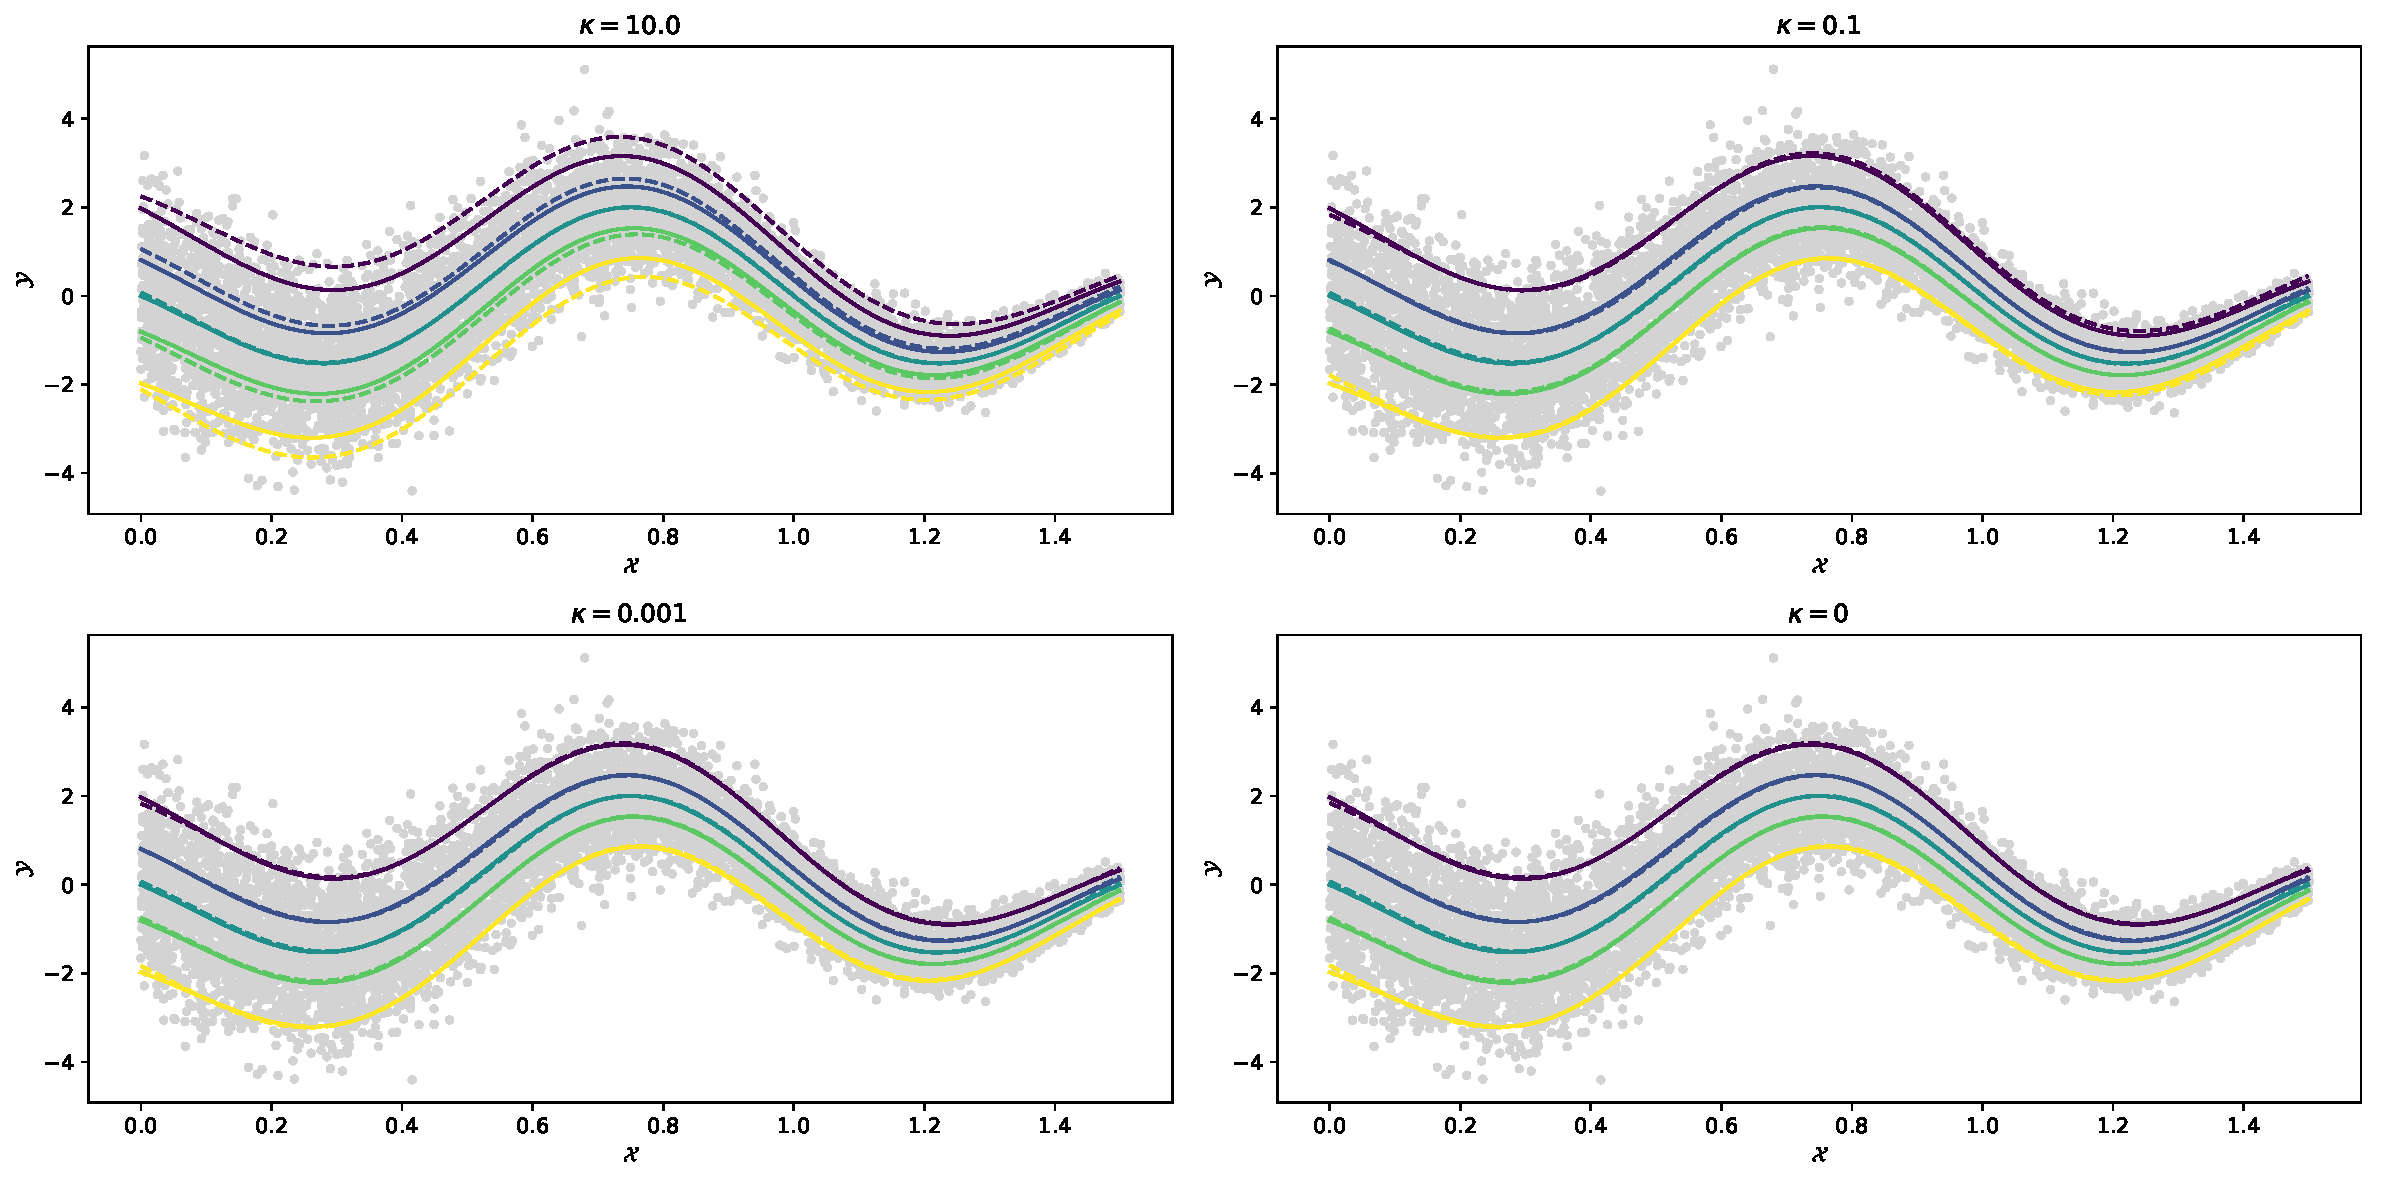
\includegraphics{src/fig/autogen/iqr_kappa.pdf}}
    \caption{Impact of the Huber loss smoothing of the pinball loss for
    differents values of $\kappa$. \label{figure:kappa_study}}
\end{figure}
\begin{table}[tb]
    \caption{Examples for objective \eqref{equation:integrated_cost}.
    $\psi_1^\kappa$, $\psi_+^\kappa$: $\kappa$-smoothed absolute value
    and positive part. $h_{x}(\hyperparameter)\defeq h(x)(\theta)$.
    \label{table:integrated_risks}}
    \begin{center}
      \addtolength{\tabcolsep}{-3pt}
      \renewcommand{\arraystretch}{0.8}
        \begin{tiny}
            \begin{sc}
                \resizebox{\textwidth}{!}{%
                \begin{tabular}{lll}
                    \toprule
                    & loss & penalty \\
                    \midrule
                    Quantile  & $\displaystyle\int_{\closedinterval{0}{1}}
                    \abs{\hyperparameter - \indicator{\reals_{-}}(y -
                    h_x(\hyperparameter))}\abs{y - h_x(\hyperparameter)}
                    d\mu(\hyperparameter)$ &
                    $\lambda_{nc}\int_{\closedinterval{0}{1}}
                    \abs{-\frac{dh_x}{d\hyperparameter}(\hyperparameter)}_+
                    d\mu(\hyperparameter) +
                    \frac{\lambda}{2}\norm{h}_{\mcH_K}^2$ \\
                    M-Quantile (smooth)  &
                    $\displaystyle\int_{\closedinterval{0}{1}}
                    \abs{\hyperparameter - \indicator{\reals_{-}}(y -
                    h_x(\hyperparameter))}\psi_1^\kappa\left(y -
                    h_x(\hyperparameter)\right)d\mu(\hyperparameter)$ &
                    $\lambda_{nc}\int_{(0, 1)} \psi_+^\kappa\left(-
                    \frac{dh_x}{d\hyperparameter}(\hyperparameter)\right)
                    d\mu(\hyperparameter) +
                    \frac{\lambda}{2}\norm{h}_{\mcH_K}^2$ \\
                    Expectiles (smooth) &
                    $\displaystyle\int_{\closedinterval{0}{1}}
                    \abs{\hyperparameter - \indicator{\reals_{-}}(y -
                    h_x(\hyperparameter))}\left(y -
                    h_x(\hyperparameter)\right)^2d\mu(\hyperparameter)$ &
                    $\lambda_{nc} \int_{(0, 1)}
                    \abs{-\frac{dh_x}{d\hyperparameter}(\hyperparameter)}_+^2
                    d\mu(\hyperparameter) +
                    \frac{\lambda}{2}\norm{h}_{\mcH_K}^2$ \\
                    Cost-Sensitive & $\displaystyle\int_{
                    \closedinterval{-1}{1}} \abs{\frac{\hyperparameter + 1}{2}
                    - \indicator{\{-1\}}(y)}\abs{1 -
                    yh_{x}(\hyperparameter)}_{+} d\mu(\theta)$ & $
                    \frac{\lambda}{2}\norm{h}_{\mcH_K}^2$ \\
                    Cost-Sensitive (smooth) &
                    $\displaystyle\int_{\closedinterval{-1}{1}}
                    \abs{\frac{\hyperparameter + 1}{2} -
                    \indicator{\{-1\}}(y)}\psi_+^\kappa\left(1 -
                    yh_{x}(\hyperparameter)\right) d\mu(\theta)$ & $
                    \frac{\lambda}{2}\norm{h}_{\mcH_K}^2$ \\
                    Level-Set   &
                    $\displaystyle\int_{\closedinterval{\epsilon}{1}}
                    -t(\hyperparameter) +
                    \frac{1}{\theta}\abs{t(\hyperparameter) -
                    h_x(\hyperparameter)}_+
                    d\mu(\hyperparameter)$ & $
                    \frac{1}{2}\displaystyle\int_{
                    \closedinterval{\epsilon}{1}}
                    \norm{h(\cdot)(\hyperparameter)}_{
                    \mcH_{k_{\inputspace}}}^2 d\mu(\hyperparameter) +
                    \frac{\lambda}{2}\norm{t}_{\mcH_{k_b}}^2$\\ \bottomrule
                \end{tabular}}
            \end{sc}
        \end{tiny}
        \addtolength{\tabcolsep}{3pt}
        \renewcommand{\arraystretch}{0.8}
    \end{center}
\end{table}
%
\subsection{Experimental protocol for \ac{QR}}  \label{subsection:proto_exp} In
this section, we give additional details regarding the choices being made while
implementing the \ac{ITL} method for $\infty$-\ac{QR}.
%
%\paragraph{Crossing Quantiles}
%The model was trained with a
%bias.  For $k_{\inputspace}$ a Gaussian kernel was used,
%$k_{\hyperparameterspace}$ and $k_{b}$ were Laplacian kernels. All bandwidths
%were set to $10$ to emphasise the possible crossings.

%\begin{dmath}\label{equation:non_crossing_constraint}
    %\Omega(h) = \lambda_{c}\sum_{i=1}^N \int_{(0, 1)} \abs{
    %-\frac{\partial}{\partial \tau} h_{\tau}(X_i)}_+ d\mu(\tau) +
    %\frac{\lambda}{2}(\norm{f}_{K}^2 + \norm{b}_{kb}^2).
%\end{dmath}
%Note that if the integral in \cref{equation:non_crossing_constraint} in uses
%the same samples $\tau_j$'s as the one used to approximate the cost function
%$\cost$, then the representer theorem applies with the expansion given in
%\cref{equation:expanded_non_crossing_constraint}.
%\begin{dmath}\label{equation:expanded_non_crossing_constraint}
    %\Omega_\lambda(h)=\lambda\sum_{j=1}^T\sum_{i=1}^N \abs{-\sum_{j'=1}^T
    %\sum_{i'=1}^N\alpha_{i'j'} k_{\inputspace}(x_i, x_{i'})\frac{\partial
    %k_{\hyperparameterspace}}{\partial\tau_j}(\tau_j, \tau_{j'}) -
    %\beta_j\frac{\partial k_b}{\partial \tau_j}(\tau_j, \tau_{j'})}_+ +
    %\sum_{i, i'=1}^N\sum_{j,
    %j'=1}^T\alpha_{ij}\alpha_{i'j'}k_{\inputspace}(x_i,
    %x_{i'})k_{\hyperparameterspace}(\tau_j,
    %\tau_{j'})+\beta_{j}\beta_{j'}k_b(\tau_j, \tau_{j'}).
%\end{dmath}
%\begin{center}
    %\begin{figure}[h]
        %% \resizebox{!}{.65\linewidth}{\includegraphics{fig/bias_experiment.eps}}
        %\caption{Model misspecification in quantile regression on the dataset
        %Engel. Left plot shows a linear model with bias and right plot without
        %bias.\label{figure:misspecified_models}}
    %\end{figure}
%\end{center}
%\par
%
\paragraph{\ac{QR} real datasets}
%
For $\infty$-\ac{QR}, $k_{\inputspace}$, $k_{\hyperparameterspace}$ were
Gaussian kernels. We set a bias term $k_b=k_{\hyperparameterspace}$. The
hyperparameters optimized were $\lambda$, the weight of the ridge penalty,
$\sigma_\inputspace$, the input kernel parameter, and
$\sigma_\hyperparameterspace=\sigma_b$, the output kernel parameter. They were
optimized in the (log)space of $\closedinterval{10^{-6}}{10^{6}}^3$. The
non-crossing constraint $\lambda_{nc}$ was set to $1$. The model was trained on
the continuum $\Theta=\openinterval{0}{1}$ using QMC and Sobol sequences. For
all datasets we draw $m=100$ quantiles form a Sobol sequence \par
%
For \ac{JQR} we similarly chose two Gaussian kernels. The optimized
hyperparameters were the same as for $\infty$-\ac{QR}.
% are also the bandwidth of the Gaussian kernel acting on the inputs, the bandwith
% of the kernel acting on the outputs, and the regularization tradeoff $\lambda$
% which where optimized in the (log)space $\closedinterval{10^{-6}}{10^{6}}^3$.
The quantiles learned were $\theta\in\Set{0.1, 0.3, 0.5, 0.7, 0.9}$.

For the IND-\ac{QR} baseline, we trained independently a non-paramatric
quantile estimator as described in \citet{takeuchi2006nonparametric}. A
Gaussian kernel was used and its bandwidth was optimized in the (log)space of
$\closedinterval{10^{-6}}{10^6}$. No non-crossing was enforced. \par
%
% \paragraph{Impact of the $\mcH_{k_{\hyperparameterspace}}$ kernel}
% See \cref{figure:gamma_t_study}.
% \begin{center}
%     \begin{figure}
%         % \resizebox{!}{.5\linewidth}{\includegraphics{fig/gamma_t_study.eps}}
%         \caption{Impact of the hyperparameter $\gamma_{\tau}$ on the
%         hyperparameter kernel $k_{\hyperparameterspace}$. Top row shows models
%         with a bias terms for $\gamma_{\tau}\in\Set{0.1, 100}$
%         respectfully left to right.  Bottom row shows the same for models
%         without bias.}
%     \label{figure:gamma_t_study}
%     \end{figure}
% \end{center}
\subsection{Experiments with \ac{CSC}}
\label{subsection:csc_expe}
In this section we provide numerical illustration concerning the \ac{CSC} problem.
We used the Iris \acs{UCI} dataset with $4$ attributes and $150$
samples, the two synthetic \textsc{scikit-learn}
\citep{pedregosa2011scikit} datasets \textsc{Two-Moons} (noise=$0.4$) and
$\textsc{Circles}$ (noise=$0.1$) with both $2$ attributes and $1000$
samples and a third synthetic \textsc{scikit-learn} dataset \textsc{Toy}
(class sep=$0.5$) with $20$ features ($4$ redundant and $10$ informative)
and $n=1000$ samples.\par
%
As detailed in \cref{section:infinite_tasks}, \acl{CSC} on a continuum
$\hyperparameterspace = \closedinterval{-1}{1}$ that we call \ac{ICSC}
can be tackled by our proposed technique.  In this case, the hyperparameter
$\hyperparameter$ controls the tradeoff between the importance of the correct
classification with labels $-1$ and $+1$. When $\hyperparameter = -1$,
class $-1$ is emphasized; the probability of correctly classified instances
with this label (called specificity) is desired to be $1$.  Similarly, for
$\hyperparameter = +1$, the probability of correct classification of samples
with label $+1$ (called sensitivity) is ideally $1$.\par
%
To illustrate the advantage of (infinite) joint learning we used two synthetic
datasets \textsc{Circles} and \textsc{Two-Moons} and the \acs{UCI}
\textsc{Iris} dataset. We chose $k_{\inputspace}$ to be a Gaussian kernel with
bandwidth $\sigma_{\inputspace}=(2\gamma_{\inputspace})^{(-1/2)}$ the median of
the Euclidean pairwise distances of the input points \citep{jaakkola1999using}.
$k_{\hyperparameterspace}$ is also a Gaussian kernel with bandwidth
$\gamma_{\hyperparameterspace}=5$.  We used $m=20$ for all datasets.
%
As a baseline we trained independently 3 \acl{CSC} classifiers with
$\hyperparameter\in\Set{-0.9,0, 0.9}$. We repeated $50$ times a random $50-50\%$
train-test split of the dataset and report the average test error and standard
deviation (in terms of sensitivity and specificity) \par
%
Our results are illustrated in \cref{table:csc_results}. For $\theta=-0.9$, both
 independent and joint learners give the desired $100\%$ specificity; the
joint \acl{CSC} scheme however has significantly higher sensitivity value
($15\%$ vs $0\%$) on the dataset \textsc{Circles}. Similar conclusion holds for the
$\theta=+0.9$ extreme: the ideal sensitivity is reached by both techniques, but
the joint learning scheme performs better in terms of specificity ($0\%$ vs
$12\%$) on the dataset \textsc{Circles}. \par
%
\begin{table*}[!htbp]
    \caption{\acs{ICSC} vs Independent (IND)-\acs{CSC}. Higher is
    better.\label{table:csc_results}}
    \addtolength{\tabcolsep}{-3pt}
    \renewcommand{\arraystretch}{0.8}% Tighter
    \begin{center}
        \begin{tiny}
            \begin{sc}
                \resizebox{.7\textwidth}{!}{%
                \begin{tabular}{cccccccc}
                    \toprule
                    \multirow{2}{*}{Dataset} & \multirow{2}{*}{Method} &
                    \multicolumn{2}{c}{$\theta=-0.9$} &
                    \multicolumn{2}{c}{$\theta=0$} &
                    \multicolumn{2}{c}{$\theta=+0.9$} \\
                    \cmidrule(lr){3-4} \cmidrule(lr){5-6} \cmidrule(lr){7-8} &
                    & \textsc{sensitivity} & \textsc{specificity} &
                    \textsc{sensitivity} & \textsc{specificity} &
                    \textsc{sensitivity} & \textsc{specificity} \\
                    \midrule
                    \multirow{ 2}{*}{\textsc{Two-Moons}} & IND &
                    $0.3\pm0.05$ & $0.99\pm0.01$ & $0.83\pm0.03$ &
                    $0.86\pm0.03$ & $0.99\pm0$ & $0.32\pm0.06$ \\
                                                & \acs{ICSC} & $0.32\pm0.05$ &
                    $0.99\pm0.01$ & $0.84\pm0.03$ & $0.87\pm0.03$ & $1\pm0$ &
                    $0.36\pm0.04$  \\
                    \multirow{ 2}{*}{\textsc{Circles}} & IND & $0\pm0$
                    & $1\pm0$ & $0.82\pm0.02$ & $0.84\pm0.03$ & $1\pm0$ &
                    $0\pm0$ \\
                                              & \acs{ICSC} & $0.15\pm0.05$ &
                    $1\pm0$ & $0.82\pm0.02$ & $0.84\pm0.03$ & $1\pm0$ &
                    $0.12\pm0.05$  \\
                    \multirow{ 2}{*}{\textsc{Iris}} & IND &
                    $0.88\pm0.08$ & $ 0.94\pm0.06$ & $0.94\pm0.05$ &
                    $0.92\pm0.06$ & $0.97\pm0.05$ & $0.87\pm0.06$\\
                                           & \acs{ICSC} & $0.89\pm0.08$ &
                    $0.94\pm0.05$ & $0.94\pm0.06$ & $0.92\pm0.05$ &
                    $0.97\pm0.04$ & $0.90\pm0.05$
                    \\
                    \multirow{ 2}{*}{\textsc{Toy}} & IND &
                    $0.51\pm0.06$ & $ 0.98\pm0.01$ & $0.83\pm0.03$ &
                    $0.86\pm0.03$ & $0.97\pm0.01$ & $0.49\pm0.07$\\
                                           & \acs{ICSC} & $0.63\pm0.04$ &
                    $0.96\pm0.01$ & $0.83\pm0.03$ & $0.85\pm0.03$ &
                    $0.95\pm0.02$ & $0.61\pm0.04$
                    \\
                    \bottomrule
                \end{tabular}}
            \end{sc}
        \end{tiny}
    \end{center}
    \addtolength{\tabcolsep}{3pt}
    \renewcommand{\arraystretch}{1.0}% Tighter
\end{table*}
% \subsubsection{Illustration of the \ac{CSC} datasets}
% \begin{figure}[!htbp]
% \setlength\fboxsep{0pt}\setlength\fboxrule{0.75pt}
% \ffigbox[\textwidth]
% {
% \begin{subfloatrow}[2]
% %\fbox{
% \ffigbox[.49\textwidth]
%   {
%     \caption{\textsc{Circle} dataset}
%     \label{subfigure:csc_circle}
%   }
%   {
%     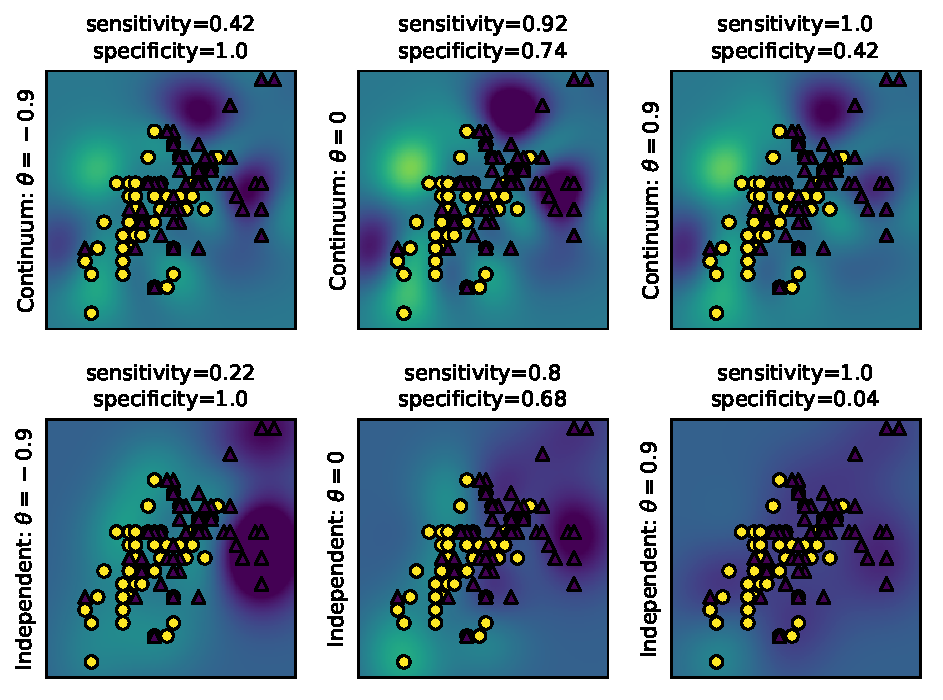
\includegraphics[angle=-90,width=\linewidth]{src/fig/autogen/icsl_vs.pdf}%
%   }
% %}
% %\fbox{
% \ffigbox[.4825\textwidth]
%   {
%     \caption{\textsc{Two-Moons} dataset}
%     \label{subfigure:csc_moons}
%   }
%   {
%     \includegraphics[angle=-90,width=\linewidth]{src/fig/autogen/icsl_vs_moons.pdf}%
%   }
% %}
% \end{subfloatrow}%
% }
% {
%     \caption{Illustration of some datasets used in \cref{table:csc_results}.
%     \label{figure:csc_datasets}}
% }
% \end{figure}%
% \textsc{Two-Moons} and \textsc{Circles} used in \cref{table:csc_results}.

\printbibliography[heading=subbibliography]
\end{refsection}
%\ifthenelse{\NOT\isundefined{\draft}\OR\NOT\isundefined{\final}}{
    %\subsubsection*{Acronyms}
    %\printacronyms[heading=none]
%}{}
%

%\section{Additional Experiments}
%We present here more details on the experimental protocol used in the main
paper as well as new experiments.
\subsection{Alternative hyperparameters sampling}\label{subsection:sampling}
Many quadrature rules such as \ac{MC} and \ac{QMC} methods are well suited for
\acl{ITL}. For instance when $\hyperparameterspace$ is high dimensional,
\ac{MC} is typically prefered over \ac{QMC}, and vice versa. If
$\hyperparameterspace$ is one dimensional and the function to integrate is
smooth enough then a Gauss-Legendre quadrature would be preferable. In
\cref{sec:V} of the main paper we provide a unified notation to handle
\ac{MC}, \ac{QMC} and other quadrature rules. In the case of
\begin{itemize}
    \item \ac{MC}: $w_j = \frac{1}{m}$ and $(\theta_j)_{j=1}^m
    \sim \mu^{\otimes m}$.
    %Note that if $\mu=\delta_{\theta_j'}$ is a dirac measure  centered at
    %$\theta_{j'}$ then $\theta_j=\theta_j'$.
    \item \ac{QMC}: $w_j = m^{-1}F^{-1}(\theta_j)$ and $(\theta_j)_{j=1}^m$
    is a sequence with values in $[0, 1]^d$ such as the % uniform properties
    Sobol or Halton sequence, $\mu$ is assumed to be absolutely continuous
    \acs{wrt} the Lebesgue measure, $F$ is the associated cdf.
    \item Quadrature rules: $((\theta_j, w'_j))_{j=1}^m$ is the indexed set of
    locations and weights produced by the quadrature rule, $w_j
    = w'_j f_{\mu}(\theta_j)$, $\mu$ is assumed to be absolutely continuous
    \acs{wrt} the Lebesgue measure, and $f_\mu$ denotes its corresponding
    probability density function.
\end{itemize}
\subsection{Impact of the number of hyperparameters sampled}
\begin{figure}[!htbp]
    \centering
    \includegraphics[width=\textwidth]{src/fig/autogen/iqr_m.pdf}
    \caption{Impact of the number of hyperparameters sampled.
             \label{figure:iqr_m}}
\end{figure}
In the experiment presented on \cref{figure:iqr_m}, on the sine synthetic
benchmark, we draw $n=1000$ training points and study the impact of increasing
$m$ on the quality of the quantiles at $\theta\in\Set{0.05, 0.25, 0.5, 0.75,
0.95}$. We notice that when $m\ge34\approx\sqrt{1000}$ there is little benefit
to draw more $m$ samples are the quantile curves do not change on the
$n_{\text{test}}=2000$ test points.
\subsection{Smoothifying the cost function} \label{subsection:infimal_convo}
The resulting $\kappa$-smoothed ($\kappa\in\reals_+$) absolute value
($\psi_{1}^\kappa$) and positive part ($\psi_{+}^\kappa$) are as follows:
\begin{align*}
  \psi_{1}^\kappa(p) &\defeq \left(\kappa \abs{\cdot} \square \frac{1}{2}
    \abs{\cdot}^2 \right)(p)
     =
     \begin{cases}
        \frac{1}{2\kappa}p^2 & \text{if $\abs{p} \le \kappa$} \\
        \abs{p} - \frac{\kappa}{2} & \text{otherwise},
    \end{cases}\\
     \psi_{+}^\kappa(p) &\defeq \left(\kappa\abs{\cdot}_+ \square\frac{1}{2}
     \abs{\cdot}^2 \right)(p) =
     \begin{cases}
         \frac{1}{2\kappa}\abs{p}_+^2 & \text{if $p \le \kappa$} \\
         p - \frac{\kappa}{2} & \text{otherwise.}
     \end{cases}
\end{align*}
where $\square$ is the classical infimal convolution \citep{bauschke2011convex}.
All the smoothified loss functions used in this paper
have been gathered in \cref{table:integrated_risks}.
\paragraph{Remarks}
\begin{itemize}[labelindent=0cm,leftmargin=*,topsep=0cm,partopsep=0cm,
                parsep=0cm,itemsep=0cm]
    \item Minimizing the $\kappa$-smoothed pinball loss
    \begin{align*}
     \parametrizedcost{\hyperparameter,\kappa}(y, h(x))=\abs{\hyperparameter -
     \indicator{\reals_{-}}(y - h(x))}\psi_1^\kappa(y - h(x)),
    \end{align*}
    yields the quantiles when $\kappa\rightarrow 0$, the expectiles as
    $\kappa\to+\infty$. The intermediate values are known as M-quantiles
    \citep{breckling1988m}.
    \item In practice, the absolute value and positive part can be approximated
    by a smooth function by setting the smoothing parameter $\kappa$ to be a
    small positive value;
    % \rb{or even zero}
    the optimization showed a robust behaviour \acs{wrt} this choice with a
    random coefficient initialization.
    % \rb{as    pointed out by \citet{lewis2013nonsmooth}}.
%     \item the cost of evaluating the model $h$ one $n$ samples and $m$
%     hyperparameters is $\mathcal{O}(n^2m + m^2n)$ and it takes
%     $\mathcal{O}(m^2+n^2)$ to fit in memory.
\end{itemize}\par
\paragraph{Impact of the Huber loss support}
The influence of the $\kappa$ parameter is illustrated in
\cref{figure:kappa_study}.  For this experiment, $10000$ samples have been
generated from the sine wave dataset described in \cref{paragraph:datasets},
and the model have been trained on $100$ quantiles generated from a
Gauss-Legendre Quadrature.  When $\kappa$ is large the expectiles are learnt
(dashed lines) while when $\kappa$ is small the quantiles are recovered (the
dashed lines on the right plot match the theoretical quantiles in plain lines).
It took $225$s ($258$ iteration, and $289$ function evaluations) to train
for $\kappa=1\cdot 10^1$, $1313$s for $\kappa=1\cdot 10^{-1}$ ($1438$
iterations and $1571$ function evaluations), $931$s for $\kappa=1e^{-3}$
($1169$ iterations and $1271$ function evaluations) and $879$s for $\kappa=0$
($1125$ iterations and $1207$ function evaluations). We used a GPU Tensorflow
implementation and run the experiments in float64 on a computer equipped with a
GTX $1070$, and intel i7 $7700$ and $16$GB of DRAM.
\begin{figure}[!htbp]
    \centering
    \resizebox{!}{.5\linewidth}{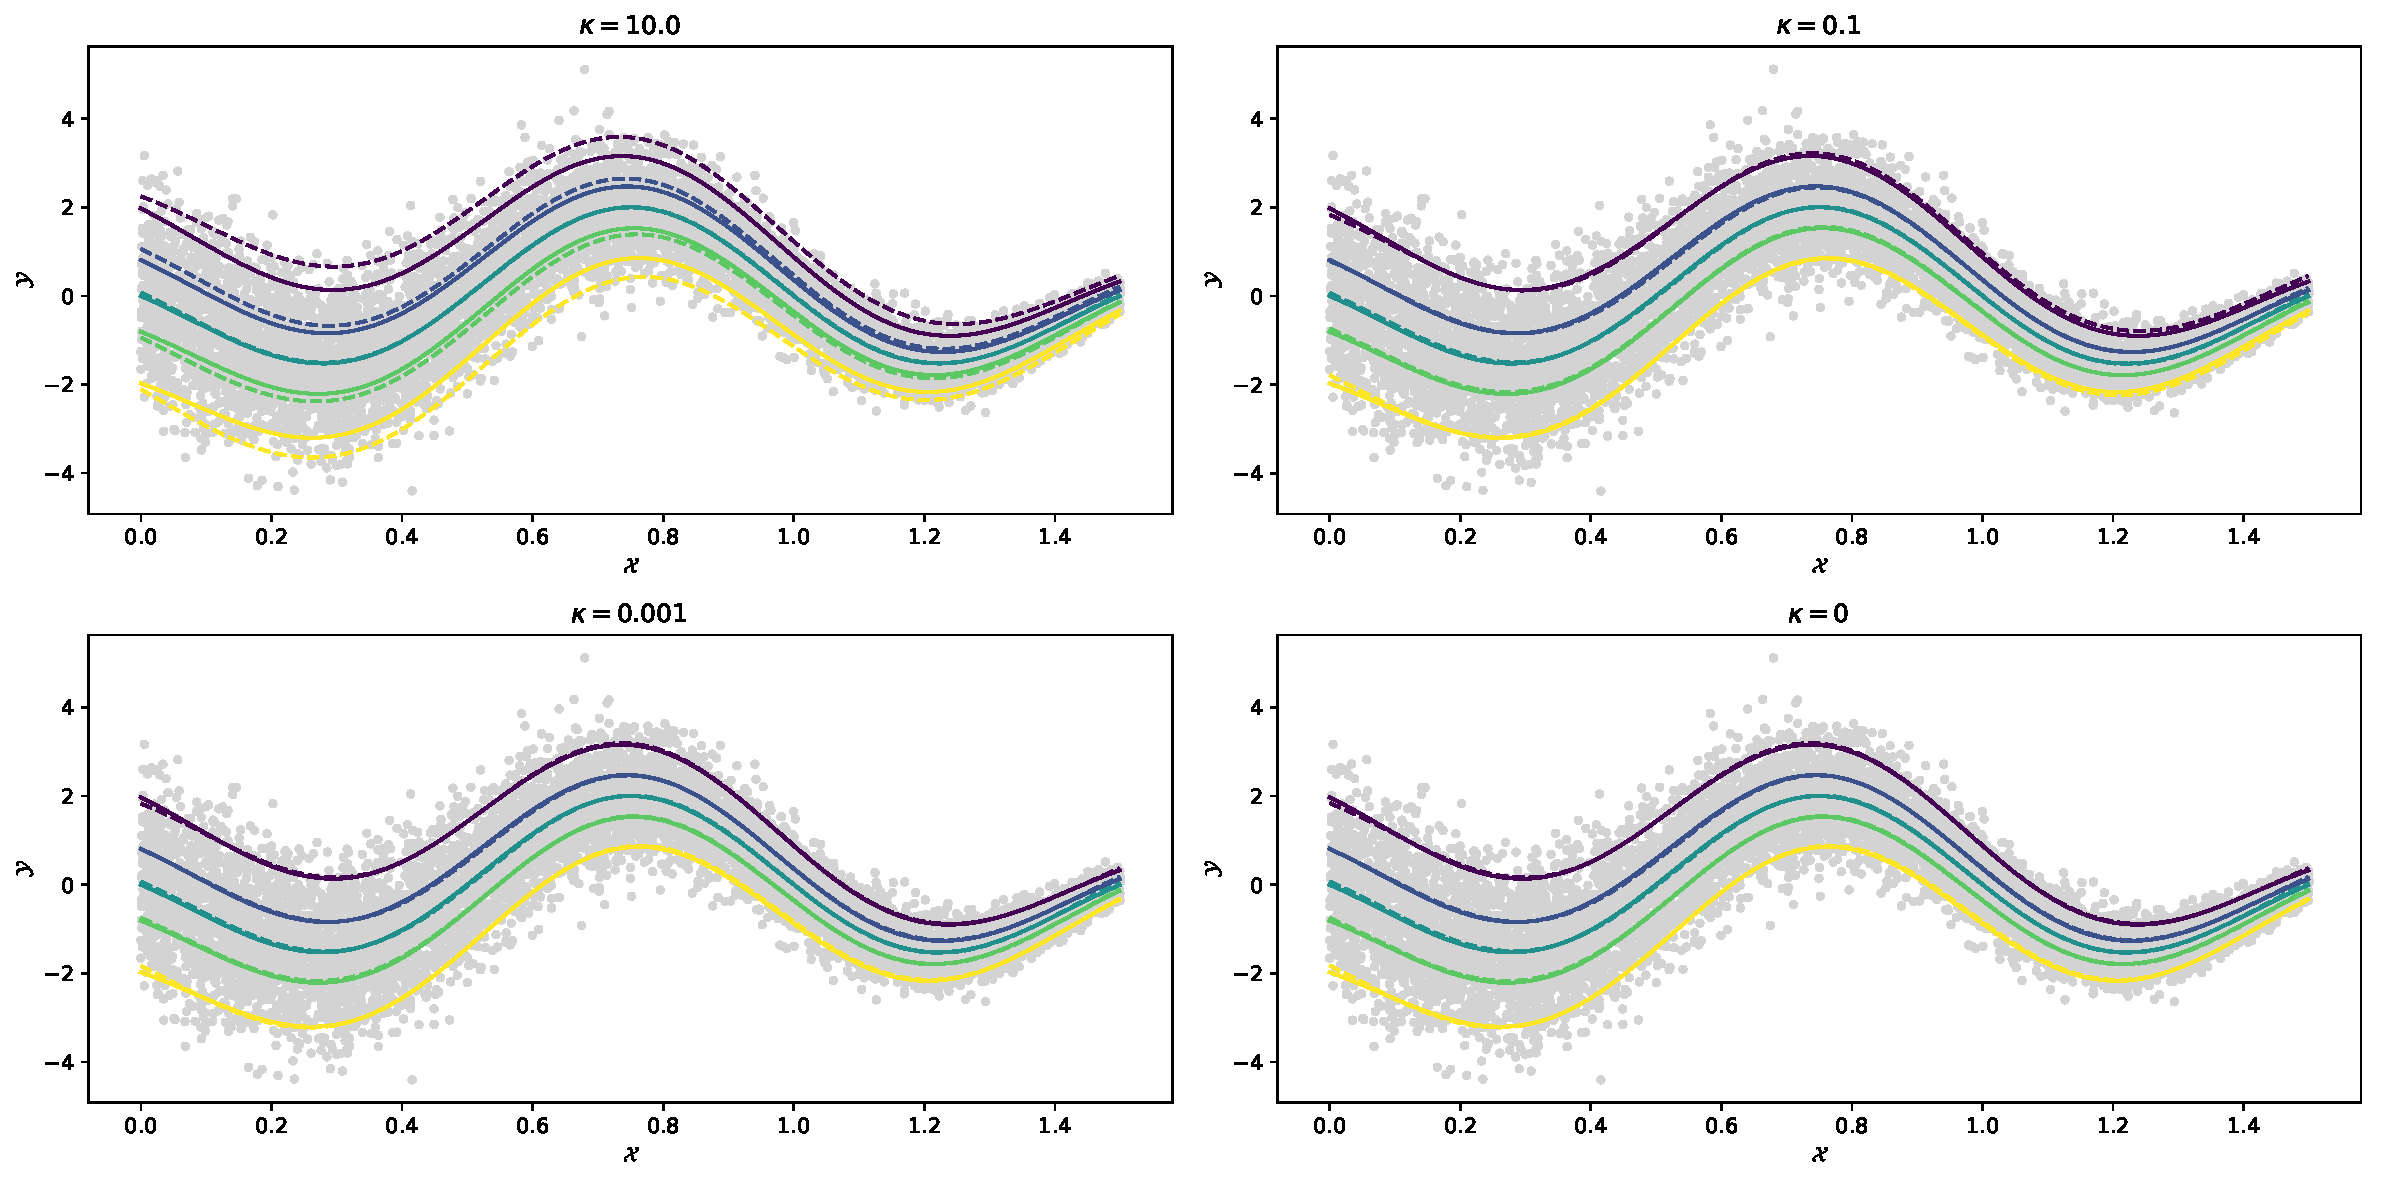
\includegraphics{src/fig/autogen/iqr_kappa.pdf}}
    \caption{Impact of the Huber loss smoothing of the pinball loss for
    differents values of $\kappa$. \label{figure:kappa_study}}
\end{figure}
\begin{table}[tb]
    \caption{Examples for objective \eqref{equation:integrated_cost}.
    $\psi_1^\kappa$, $\psi_+^\kappa$: $\kappa$-smoothed absolute value
    and positive part. $h_{x}(\hyperparameter)\defeq h(x)(\theta)$.
    \label{table:integrated_risks}}
    \begin{center}
      \addtolength{\tabcolsep}{-3pt}
      \renewcommand{\arraystretch}{0.8}
        \begin{tiny}
            \begin{sc}
                \resizebox{\textwidth}{!}{%
                \begin{tabular}{lll}
                    \toprule
                    & loss & penalty \\
                    \midrule
                    Quantile  & $\displaystyle\int_{\closedinterval{0}{1}}
                    \abs{\hyperparameter - \indicator{\reals_{-}}(y -
                    h_x(\hyperparameter))}\abs{y - h_x(\hyperparameter)}
                    d\mu(\hyperparameter)$ &
                    $\lambda_{nc}\int_{\closedinterval{0}{1}}
                    \abs{-\frac{dh_x}{d\hyperparameter}(\hyperparameter)}_+
                    d\mu(\hyperparameter) +
                    \frac{\lambda}{2}\norm{h}_{\mcH_K}^2$ \\
                    M-Quantile (smooth)  &
                    $\displaystyle\int_{\closedinterval{0}{1}}
                    \abs{\hyperparameter - \indicator{\reals_{-}}(y -
                    h_x(\hyperparameter))}\psi_1^\kappa\left(y -
                    h_x(\hyperparameter)\right)d\mu(\hyperparameter)$ &
                    $\lambda_{nc}\int_{(0, 1)} \psi_+^\kappa\left(-
                    \frac{dh_x}{d\hyperparameter}(\hyperparameter)\right)
                    d\mu(\hyperparameter) +
                    \frac{\lambda}{2}\norm{h}_{\mcH_K}^2$ \\
                    Expectiles (smooth) &
                    $\displaystyle\int_{\closedinterval{0}{1}}
                    \abs{\hyperparameter - \indicator{\reals_{-}}(y -
                    h_x(\hyperparameter))}\left(y -
                    h_x(\hyperparameter)\right)^2d\mu(\hyperparameter)$ &
                    $\lambda_{nc} \int_{(0, 1)}
                    \abs{-\frac{dh_x}{d\hyperparameter}(\hyperparameter)}_+^2
                    d\mu(\hyperparameter) +
                    \frac{\lambda}{2}\norm{h}_{\mcH_K}^2$ \\
                    Cost-Sensitive & $\displaystyle\int_{
                    \closedinterval{-1}{1}} \abs{\frac{\hyperparameter + 1}{2}
                    - \indicator{\{-1\}}(y)}\abs{1 -
                    yh_{x}(\hyperparameter)}_{+} d\mu(\theta)$ & $
                    \frac{\lambda}{2}\norm{h}_{\mcH_K}^2$ \\
                    Cost-Sensitive (smooth) &
                    $\displaystyle\int_{\closedinterval{-1}{1}}
                    \abs{\frac{\hyperparameter + 1}{2} -
                    \indicator{\{-1\}}(y)}\psi_+^\kappa\left(1 -
                    yh_{x}(\hyperparameter)\right) d\mu(\theta)$ & $
                    \frac{\lambda}{2}\norm{h}_{\mcH_K}^2$ \\
                    Level-Set   &
                    $\displaystyle\int_{\closedinterval{\epsilon}{1}}
                    -t(\hyperparameter) +
                    \frac{1}{\theta}\abs{t(\hyperparameter) -
                    h_x(\hyperparameter)}_+
                    d\mu(\hyperparameter)$ & $
                    \frac{1}{2}\displaystyle\int_{
                    \closedinterval{\epsilon}{1}}
                    \norm{h(\cdot)(\hyperparameter)}_{
                    \mcH_{k_{\inputspace}}}^2 d\mu(\hyperparameter) +
                    \frac{\lambda}{2}\norm{t}_{\mcH_{k_b}}^2$\\ \bottomrule
                \end{tabular}}
            \end{sc}
        \end{tiny}
        \addtolength{\tabcolsep}{3pt}
        \renewcommand{\arraystretch}{0.8}
    \end{center}
\end{table}
%
\subsection{Experimental protocol for \ac{QR}}  \label{subsection:proto_exp} In
this section, we give additional details regarding the choices being made while
implementing the \ac{ITL} method for $\infty$-\ac{QR}.
%
%\paragraph{Crossing Quantiles}
%The model was trained with a
%bias.  For $k_{\inputspace}$ a Gaussian kernel was used,
%$k_{\hyperparameterspace}$ and $k_{b}$ were Laplacian kernels. All bandwidths
%were set to $10$ to emphasise the possible crossings.

%\begin{dmath}\label{equation:non_crossing_constraint}
    %\Omega(h) = \lambda_{c}\sum_{i=1}^N \int_{(0, 1)} \abs{
    %-\frac{\partial}{\partial \tau} h_{\tau}(X_i)}_+ d\mu(\tau) +
    %\frac{\lambda}{2}(\norm{f}_{K}^2 + \norm{b}_{kb}^2).
%\end{dmath}
%Note that if the integral in \cref{equation:non_crossing_constraint} in uses
%the same samples $\tau_j$'s as the one used to approximate the cost function
%$\cost$, then the representer theorem applies with the expansion given in
%\cref{equation:expanded_non_crossing_constraint}.
%\begin{dmath}\label{equation:expanded_non_crossing_constraint}
    %\Omega_\lambda(h)=\lambda\sum_{j=1}^T\sum_{i=1}^N \abs{-\sum_{j'=1}^T
    %\sum_{i'=1}^N\alpha_{i'j'} k_{\inputspace}(x_i, x_{i'})\frac{\partial
    %k_{\hyperparameterspace}}{\partial\tau_j}(\tau_j, \tau_{j'}) -
    %\beta_j\frac{\partial k_b}{\partial \tau_j}(\tau_j, \tau_{j'})}_+ +
    %\sum_{i, i'=1}^N\sum_{j,
    %j'=1}^T\alpha_{ij}\alpha_{i'j'}k_{\inputspace}(x_i,
    %x_{i'})k_{\hyperparameterspace}(\tau_j,
    %\tau_{j'})+\beta_{j}\beta_{j'}k_b(\tau_j, \tau_{j'}).
%\end{dmath}
%\begin{center}
    %\begin{figure}[h]
        %% \resizebox{!}{.65\linewidth}{\includegraphics{fig/bias_experiment.eps}}
        %\caption{Model misspecification in quantile regression on the dataset
        %Engel. Left plot shows a linear model with bias and right plot without
        %bias.\label{figure:misspecified_models}}
    %\end{figure}
%\end{center}
%\par
%
\paragraph{\ac{QR} real datasets}
%
For $\infty$-\ac{QR}, $k_{\inputspace}$, $k_{\hyperparameterspace}$ were
Gaussian kernels. We set a bias term $k_b=k_{\hyperparameterspace}$. The
hyperparameters optimized were $\lambda$, the weight of the ridge penalty,
$\sigma_\inputspace$, the input kernel parameter, and
$\sigma_\hyperparameterspace=\sigma_b$, the output kernel parameter. They were
optimized in the (log)space of $\closedinterval{10^{-6}}{10^{6}}^3$. The
non-crossing constraint $\lambda_{nc}$ was set to $1$. The model was trained on
the continuum $\Theta=\openinterval{0}{1}$ using QMC and Sobol sequences. For
all datasets we draw $m=100$ quantiles form a Sobol sequence \par
%
For \ac{JQR} we similarly chose two Gaussian kernels. The optimized
hyperparameters were the same as for $\infty$-\ac{QR}.
% are also the bandwidth of the Gaussian kernel acting on the inputs, the bandwith
% of the kernel acting on the outputs, and the regularization tradeoff $\lambda$
% which where optimized in the (log)space $\closedinterval{10^{-6}}{10^{6}}^3$.
The quantiles learned were $\theta\in\Set{0.1, 0.3, 0.5, 0.7, 0.9}$.

For the IND-\ac{QR} baseline, we trained independently a non-paramatric
quantile estimator as described in \citet{takeuchi2006nonparametric}. A
Gaussian kernel was used and its bandwidth was optimized in the (log)space of
$\closedinterval{10^{-6}}{10^6}$. No non-crossing was enforced. \par
%
% \paragraph{Impact of the $\mcH_{k_{\hyperparameterspace}}$ kernel}
% See \cref{figure:gamma_t_study}.
% \begin{center}
%     \begin{figure}
%         % \resizebox{!}{.5\linewidth}{\includegraphics{fig/gamma_t_study.eps}}
%         \caption{Impact of the hyperparameter $\gamma_{\tau}$ on the
%         hyperparameter kernel $k_{\hyperparameterspace}$. Top row shows models
%         with a bias terms for $\gamma_{\tau}\in\Set{0.1, 100}$
%         respectfully left to right.  Bottom row shows the same for models
%         without bias.}
%     \label{figure:gamma_t_study}
%     \end{figure}
% \end{center}
\subsection{Experiments with \ac{CSC}}
\label{subsection:csc_expe}
In this section we provide numerical illustration concerning the \ac{CSC} problem.
We used the Iris \acs{UCI} dataset with $4$ attributes and $150$
samples, the two synthetic \textsc{scikit-learn}
\citep{pedregosa2011scikit} datasets \textsc{Two-Moons} (noise=$0.4$) and
$\textsc{Circles}$ (noise=$0.1$) with both $2$ attributes and $1000$
samples and a third synthetic \textsc{scikit-learn} dataset \textsc{Toy}
(class sep=$0.5$) with $20$ features ($4$ redundant and $10$ informative)
and $n=1000$ samples.\par
%
As detailed in \cref{section:infinite_tasks}, \acl{CSC} on a continuum
$\hyperparameterspace = \closedinterval{-1}{1}$ that we call \ac{ICSC}
can be tackled by our proposed technique.  In this case, the hyperparameter
$\hyperparameter$ controls the tradeoff between the importance of the correct
classification with labels $-1$ and $+1$. When $\hyperparameter = -1$,
class $-1$ is emphasized; the probability of correctly classified instances
with this label (called specificity) is desired to be $1$.  Similarly, for
$\hyperparameter = +1$, the probability of correct classification of samples
with label $+1$ (called sensitivity) is ideally $1$.\par
%
To illustrate the advantage of (infinite) joint learning we used two synthetic
datasets \textsc{Circles} and \textsc{Two-Moons} and the \acs{UCI}
\textsc{Iris} dataset. We chose $k_{\inputspace}$ to be a Gaussian kernel with
bandwidth $\sigma_{\inputspace}=(2\gamma_{\inputspace})^{(-1/2)}$ the median of
the Euclidean pairwise distances of the input points \citep{jaakkola1999using}.
$k_{\hyperparameterspace}$ is also a Gaussian kernel with bandwidth
$\gamma_{\hyperparameterspace}=5$.  We used $m=20$ for all datasets.
%
As a baseline we trained independently 3 \acl{CSC} classifiers with
$\hyperparameter\in\Set{-0.9,0, 0.9}$. We repeated $50$ times a random $50-50\%$
train-test split of the dataset and report the average test error and standard
deviation (in terms of sensitivity and specificity) \par
%
Our results are illustrated in \cref{table:csc_results}. For $\theta=-0.9$, both
 independent and joint learners give the desired $100\%$ specificity; the
joint \acl{CSC} scheme however has significantly higher sensitivity value
($15\%$ vs $0\%$) on the dataset \textsc{Circles}. Similar conclusion holds for the
$\theta=+0.9$ extreme: the ideal sensitivity is reached by both techniques, but
the joint learning scheme performs better in terms of specificity ($0\%$ vs
$12\%$) on the dataset \textsc{Circles}. \par
%
\begin{table*}[!htbp]
    \caption{\acs{ICSC} vs Independent (IND)-\acs{CSC}. Higher is
    better.\label{table:csc_results}}
    \addtolength{\tabcolsep}{-3pt}
    \renewcommand{\arraystretch}{0.8}% Tighter
    \begin{center}
        \begin{tiny}
            \begin{sc}
                \resizebox{.7\textwidth}{!}{%
                \begin{tabular}{cccccccc}
                    \toprule
                    \multirow{2}{*}{Dataset} & \multirow{2}{*}{Method} &
                    \multicolumn{2}{c}{$\theta=-0.9$} &
                    \multicolumn{2}{c}{$\theta=0$} &
                    \multicolumn{2}{c}{$\theta=+0.9$} \\
                    \cmidrule(lr){3-4} \cmidrule(lr){5-6} \cmidrule(lr){7-8} &
                    & \textsc{sensitivity} & \textsc{specificity} &
                    \textsc{sensitivity} & \textsc{specificity} &
                    \textsc{sensitivity} & \textsc{specificity} \\
                    \midrule
                    \multirow{ 2}{*}{\textsc{Two-Moons}} & IND &
                    $0.3\pm0.05$ & $0.99\pm0.01$ & $0.83\pm0.03$ &
                    $0.86\pm0.03$ & $0.99\pm0$ & $0.32\pm0.06$ \\
                                                & \acs{ICSC} & $0.32\pm0.05$ &
                    $0.99\pm0.01$ & $0.84\pm0.03$ & $0.87\pm0.03$ & $1\pm0$ &
                    $0.36\pm0.04$  \\
                    \multirow{ 2}{*}{\textsc{Circles}} & IND & $0\pm0$
                    & $1\pm0$ & $0.82\pm0.02$ & $0.84\pm0.03$ & $1\pm0$ &
                    $0\pm0$ \\
                                              & \acs{ICSC} & $0.15\pm0.05$ &
                    $1\pm0$ & $0.82\pm0.02$ & $0.84\pm0.03$ & $1\pm0$ &
                    $0.12\pm0.05$  \\
                    \multirow{ 2}{*}{\textsc{Iris}} & IND &
                    $0.88\pm0.08$ & $ 0.94\pm0.06$ & $0.94\pm0.05$ &
                    $0.92\pm0.06$ & $0.97\pm0.05$ & $0.87\pm0.06$\\
                                           & \acs{ICSC} & $0.89\pm0.08$ &
                    $0.94\pm0.05$ & $0.94\pm0.06$ & $0.92\pm0.05$ &
                    $0.97\pm0.04$ & $0.90\pm0.05$
                    \\
                    \multirow{ 2}{*}{\textsc{Toy}} & IND &
                    $0.51\pm0.06$ & $ 0.98\pm0.01$ & $0.83\pm0.03$ &
                    $0.86\pm0.03$ & $0.97\pm0.01$ & $0.49\pm0.07$\\
                                           & \acs{ICSC} & $0.63\pm0.04$ &
                    $0.96\pm0.01$ & $0.83\pm0.03$ & $0.85\pm0.03$ &
                    $0.95\pm0.02$ & $0.61\pm0.04$
                    \\
                    \bottomrule
                \end{tabular}}
            \end{sc}
        \end{tiny}
    \end{center}
    \addtolength{\tabcolsep}{3pt}
    \renewcommand{\arraystretch}{1.0}% Tighter
\end{table*}
% \subsubsection{Illustration of the \ac{CSC} datasets}
% \begin{figure}[!htbp]
% \setlength\fboxsep{0pt}\setlength\fboxrule{0.75pt}
% \ffigbox[\textwidth]
% {
% \begin{subfloatrow}[2]
% %\fbox{
% \ffigbox[.49\textwidth]
%   {
%     \caption{\textsc{Circle} dataset}
%     \label{subfigure:csc_circle}
%   }
%   {
%     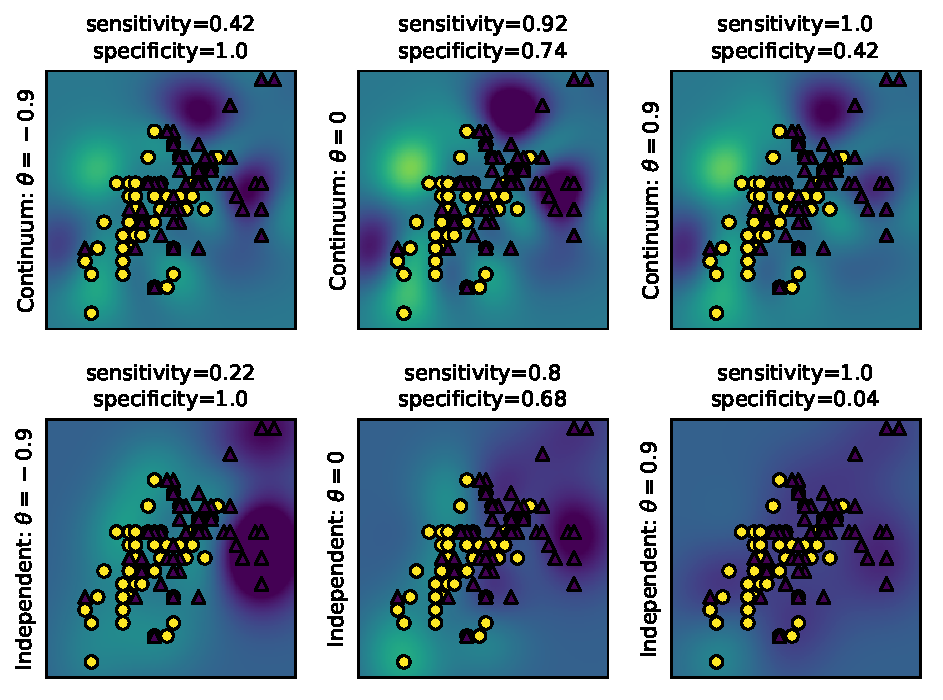
\includegraphics[angle=-90,width=\linewidth]{src/fig/autogen/icsl_vs.pdf}%
%   }
% %}
% %\fbox{
% \ffigbox[.4825\textwidth]
%   {
%     \caption{\textsc{Two-Moons} dataset}
%     \label{subfigure:csc_moons}
%   }
%   {
%     \includegraphics[angle=-90,width=\linewidth]{src/fig/autogen/icsl_vs_moons.pdf}%
%   }
% %}
% \end{subfloatrow}%
% }
% {
%     \caption{Illustration of some datasets used in \cref{table:csc_results}.
%     \label{figure:csc_datasets}}
% }
% \end{figure}%
% \textsc{Two-Moons} and \textsc{Circles} used in \cref{table:csc_results}.

